% Options for packages loaded elsewhere
\PassOptionsToPackage{unicode}{hyperref}
\PassOptionsToPackage{hyphens}{url}
%
\documentclass[
]{memoir}
\usepackage{amsmath,amssymb}
\usepackage{lmodern}
\usepackage{iftex}
\ifPDFTeX
  \usepackage[T1]{fontenc}
  \usepackage[utf8]{inputenc}
  \usepackage{textcomp} % provide euro and other symbols
\else % if luatex or xetex
  \usepackage{unicode-math}
  \defaultfontfeatures{Scale=MatchLowercase}
  \defaultfontfeatures[\rmfamily]{Ligatures=TeX,Scale=1}
  \setmainfont[]{Roboto}
  \setsansfont[]{Clancy}
  \setmonofont[Scale=0.9]{Roboto Mono}
\fi
% Use upquote if available, for straight quotes in verbatim environments
\IfFileExists{upquote.sty}{\usepackage{upquote}}{}
\IfFileExists{microtype.sty}{% use microtype if available
  \usepackage[]{microtype}
  \UseMicrotypeSet[protrusion]{basicmath} % disable protrusion for tt fonts
}{}
\makeatletter
\@ifundefined{KOMAClassName}{% if non-KOMA class
  \IfFileExists{parskip.sty}{%
    \usepackage{parskip}
  }{% else
    \setlength{\parindent}{0pt}
    \setlength{\parskip}{6pt plus 2pt minus 1pt}}
}{% if KOMA class
  \KOMAoptions{parskip=half}}
\makeatother
\usepackage{xcolor}
\usepackage{color}
\usepackage{fancyvrb}
\newcommand{\VerbBar}{|}
\newcommand{\VERB}{\Verb[commandchars=\\\{\}]}
\DefineVerbatimEnvironment{Highlighting}{Verbatim}{commandchars=\\\{\}}
% Add ',fontsize=\small' for more characters per line
\usepackage{framed}
\definecolor{shadecolor}{RGB}{248,248,248}
\newenvironment{Shaded}{\begin{snugshade}}{\end{snugshade}}
\newcommand{\AlertTok}[1]{\textcolor[rgb]{0.94,0.16,0.16}{#1}}
\newcommand{\AnnotationTok}[1]{\textcolor[rgb]{0.56,0.35,0.01}{\textbf{\textit{#1}}}}
\newcommand{\AttributeTok}[1]{\textcolor[rgb]{0.77,0.63,0.00}{#1}}
\newcommand{\BaseNTok}[1]{\textcolor[rgb]{0.00,0.00,0.81}{#1}}
\newcommand{\BuiltInTok}[1]{#1}
\newcommand{\CharTok}[1]{\textcolor[rgb]{0.31,0.60,0.02}{#1}}
\newcommand{\CommentTok}[1]{\textcolor[rgb]{0.56,0.35,0.01}{\textit{#1}}}
\newcommand{\CommentVarTok}[1]{\textcolor[rgb]{0.56,0.35,0.01}{\textbf{\textit{#1}}}}
\newcommand{\ConstantTok}[1]{\textcolor[rgb]{0.00,0.00,0.00}{#1}}
\newcommand{\ControlFlowTok}[1]{\textcolor[rgb]{0.13,0.29,0.53}{\textbf{#1}}}
\newcommand{\DataTypeTok}[1]{\textcolor[rgb]{0.13,0.29,0.53}{#1}}
\newcommand{\DecValTok}[1]{\textcolor[rgb]{0.00,0.00,0.81}{#1}}
\newcommand{\DocumentationTok}[1]{\textcolor[rgb]{0.56,0.35,0.01}{\textbf{\textit{#1}}}}
\newcommand{\ErrorTok}[1]{\textcolor[rgb]{0.64,0.00,0.00}{\textbf{#1}}}
\newcommand{\ExtensionTok}[1]{#1}
\newcommand{\FloatTok}[1]{\textcolor[rgb]{0.00,0.00,0.81}{#1}}
\newcommand{\FunctionTok}[1]{\textcolor[rgb]{0.00,0.00,0.00}{#1}}
\newcommand{\ImportTok}[1]{#1}
\newcommand{\InformationTok}[1]{\textcolor[rgb]{0.56,0.35,0.01}{\textbf{\textit{#1}}}}
\newcommand{\KeywordTok}[1]{\textcolor[rgb]{0.13,0.29,0.53}{\textbf{#1}}}
\newcommand{\NormalTok}[1]{#1}
\newcommand{\OperatorTok}[1]{\textcolor[rgb]{0.81,0.36,0.00}{\textbf{#1}}}
\newcommand{\OtherTok}[1]{\textcolor[rgb]{0.56,0.35,0.01}{#1}}
\newcommand{\PreprocessorTok}[1]{\textcolor[rgb]{0.56,0.35,0.01}{\textit{#1}}}
\newcommand{\RegionMarkerTok}[1]{#1}
\newcommand{\SpecialCharTok}[1]{\textcolor[rgb]{0.00,0.00,0.00}{#1}}
\newcommand{\SpecialStringTok}[1]{\textcolor[rgb]{0.31,0.60,0.02}{#1}}
\newcommand{\StringTok}[1]{\textcolor[rgb]{0.31,0.60,0.02}{#1}}
\newcommand{\VariableTok}[1]{\textcolor[rgb]{0.00,0.00,0.00}{#1}}
\newcommand{\VerbatimStringTok}[1]{\textcolor[rgb]{0.31,0.60,0.02}{#1}}
\newcommand{\WarningTok}[1]{\textcolor[rgb]{0.56,0.35,0.01}{\textbf{\textit{#1}}}}
\usepackage{longtable,booktabs,array}
\usepackage{calc} % for calculating minipage widths
% Correct order of tables after \paragraph or \subparagraph
\usepackage{etoolbox}
\makeatletter
\patchcmd\longtable{\par}{\if@noskipsec\mbox{}\fi\par}{}{}
\makeatother
% Allow footnotes in longtable head/foot
\IfFileExists{footnotehyper.sty}{\usepackage{footnotehyper}}{\usepackage{footnote}}
\makesavenoteenv{longtable}
\usepackage{graphicx}
\makeatletter
\def\maxwidth{\ifdim\Gin@nat@width>\linewidth\linewidth\else\Gin@nat@width\fi}
\def\maxheight{\ifdim\Gin@nat@height>\textheight\textheight\else\Gin@nat@height\fi}
\makeatother
% Scale images if necessary, so that they will not overflow the page
% margins by default, and it is still possible to overwrite the defaults
% using explicit options in \includegraphics[width, height, ...]{}
\setkeys{Gin}{width=\maxwidth,height=\maxheight,keepaspectratio}
% Set default figure placement to htbp
\makeatletter
\def\fps@figure{htbp}
\makeatother
\setlength{\emergencystretch}{3em} % prevent overfull lines
\providecommand{\tightlist}{%
  \setlength{\itemsep}{0pt}\setlength{\parskip}{0pt}}
\setcounter{secnumdepth}{5}
\usepackage{booktabs}
\usepackage{float}

\floatstyle{boxed}
\newfloat{program}{thp}{lop}
\floatname{program}{Output}

\renewcommand{\chaptername}{Module}
\renewcommand*{\chapnamefont}{\normalfont\HUGE\bfseries\sffamily}
\renewcommand*{\chapnumfont}{\normalfont\HUGE\bfseries\sffamily}
\renewcommand*{\chaptitlefont}{\normalfont\HUGE\bfseries\sffamily}

\setsecheadstyle{\sffamily}% Set \section style
\setsubsecheadstyle{\sffamily}% Set \subsection style
\setsubsubsecheadstyle{\sffamily}% Set \subsubsection style

\setlrmarginsandblock{3.5cm}{2.5cm}{*}
\setulmarginsandblock{2.5cm}{*}{1}
\checkandfixthelayout 

\raggedright
\raggedbottom
\usepackage{array}
\usepackage{caption}
\usepackage{graphicx}
\usepackage{siunitx}
\usepackage[normalem]{ulem}
\usepackage{colortbl}
\usepackage{multirow}
\usepackage{hhline}
\usepackage{calc}
\usepackage{tabularx}
\usepackage{threeparttable}
\usepackage{wrapfig}
\usepackage{adjustbox}
\usepackage{hyperref}
\ifLuaTeX
  \usepackage{selnolig}  % disable illegal ligatures
\fi
\usepackage[]{natbib}
\bibliographystyle{plainnat}
\IfFileExists{bookmark.sty}{\usepackage{bookmark}}{\usepackage{hyperref}}
\IfFileExists{xurl.sty}{\usepackage{xurl}}{} % add URL line breaks if available
\urlstyle{same} % disable monospaced font for URLs
\hypersetup{
  pdftitle={PHCM9795 Foundations of Biostatistics},
  pdfauthor={Course notes},
  hidelinks,
  pdfcreator={LaTeX via pandoc}}

\title{PHCM9795 Foundations of Biostatistics}
\author{Course notes}
\date{Term 2, 2023}

\begin{document}
\maketitle

{
\setcounter{tocdepth}{1}
\tableofcontents
}
\hypertarget{course-introduction}{%
\chapter*{Course introduction}\label{course-introduction}}
\addcontentsline{toc}{chapter}{Course introduction}

Welcome to PHCM9795 Foundations of Biostatistics.

This is an introductory course in biostatistics for postgraduate students. The course aims to provide students with core biostatistical skills to analyse and present quantitative data from different study types. These are essential skills required in your degree and throughout your career.

We hope you enjoy the course and will value your feedback and comment throughout the course.

\hypertarget{course-information}{%
\section*{Course information}\label{course-information}}
\addcontentsline{toc}{section}{Course information}

Biostatistics is a foundational discipline needed for the analysis and interpretation of quantitative information and its application to population health policy and practice.

This course is central to becoming a population health practitioner as the concepts and techniques developed in the course are fundamental to your studies and practice in population health. In this course you will develop an understanding of, and skills in, the core concepts of biostatistics that are necessary for analysis and interpretation of population health data and health literature.

In designing this course, we provide a learning sequence that will allow you to obtain the required graduate capabilities identified for your program. This course is taught with an emphasis on formulating a hypothesis and quantifying the evidence in relation to a specific research question. You will have the opportunity to analyse data from different study types commonly seen in population health research.

The course will allow those of you who have covered some of this material in your undergraduate and other professional education to consolidate your knowledge and skills. Students exposed to biostatistics for the first time may find the course challenging at times. Based on student feedback, the key to success in this course is to devote time to it every week. We recommend that you spend an average of 10-15 hours per week on the course, including the time spent reading the course notes and readings, listening to lectures, and working through learning activities and completing your assessments. Please use the resources provided to assist you, including online support.

\hypertarget{units-of-credit}{%
\section*{Units of credit}\label{units-of-credit}}
\addcontentsline{toc}{section}{Units of credit}

This course is a core course of the Master of Public Health, Master of Global Health and Master of Infectious Diseases Intelligence programs and associated dual degrees, comprising 6 units of credit towards the total required for completion of the study program. A value of 6 UOC requires a minimum of 150 hours work for the average student across the term.

\hypertarget{course-aim}{%
\section*{Course aim}\label{course-aim}}
\addcontentsline{toc}{section}{Course aim}

This course aims to provide students with the core biostatistical skills to apply appropriate statistical techniques to analyse and present population health data.

\hypertarget{learning-outcomes}{%
\section*{Learning outcomes}\label{learning-outcomes}}
\addcontentsline{toc}{section}{Learning outcomes}

On successful completion of this course, you will be able to:

\begin{enumerate}
\def\labelenumi{\arabic{enumi}.}
\tightlist
\item
  Summarise and visualise data using statistical software.
\item
  Demonstrate an understanding of statistical inference by interpreting p-values and confidence intervals.
\item
  Apply appropriate statistical tests for different types of variables given a research question, and interpret computer output of these tests appropriately.
\item
  Determine the appropriate sample size when planning a research study.
\item
  Present and interpret statistical findings appropriate for a population health audience.
\end{enumerate}

\hypertarget{changelog}{%
\subsection*{Changelog}\label{changelog}}
\addcontentsline{toc}{subsection}{Changelog}

\hypertarget{correlation-and-linear-regression}{%
\chapter{Correlation and linear regression}\label{correlation-and-linear-regression}}

\hypertarget{learning-objectives}{%
\section*{Learning objectives}\label{learning-objectives}}
\addcontentsline{toc}{section}{Learning objectives}

By the end of this module you will be able to:

\begin{itemize}
\tightlist
\item
  Explore the association between two continuous variables using a scatter plot;
\item
  Estimate and interpret correlation coefficients;
\item
  Estimate and interpret parameters from a simple linear regression;
\item
  Decide whether a regression model is valid;
\item
  Test a hypothesis using regression coefficients;
\item
  Outline the concept of multiple regression and its role in investigative epidemiology.
\end{itemize}

\hypertarget{readings}{%
\section*{Readings}\label{readings}}
\addcontentsline{toc}{section}{Readings}

\citet{kirkwood_sterne01}; Chapter 10. \href{http://er1.library.unsw.edu.au/er/cgi-bin/eraccess.cgi?url=https://ebookcentral.proquest.com/lib/unsw/detail.action?docID=624728}{{[}UNSW Library Link{]}}

\citet{bland15}; Chapter 11. \href{http://er1.library.unsw.edu.au/er/cgi-bin/eraccess.cgi?url=https://ebookcentral.proquest.com/lib/unsw/detail.action?docID=5891730}{{[}UNSW Library Link{]}}

\citet{acock10}; Chapter 8.

\hypertarget{introduction}{%
\section{Introduction}\label{introduction}}

In Module 5, we saw how to test whether the means from two groups are equal - in other words, whether a continuous variable is related to a categorical variable. We often want to know how closely two continuous variables are related. For example, we may want to know how closely blood cholesterol levels are related to dietary fat intake in adult men. To measure the strength of association between two continuously distributed variables, a correlation coefficient is used.

We may also want to know how well one continuous measurement predicts the value of another continuous measurement. For example, we may want to know how well height predicts values of lung capacity in a community of adults. A regression model allows us to use one measurement to predict another measurement.

Although both correlation coefficients and regression models can be used to describe the degree of association between two continuous variables, the two methods provide very different statistical information. It is important to note that both methods only measures the strengths of an association between variables and does not imply a causal relationship.

\hypertarget{correlation}{%
\section{Correlation}\label{correlation}}

We use correlation to measure the strength of a linear relationship between two variables. Before calculating a correlation coefficient, a scatter plot should first be obtained to give an understanding of the nature of the relationship between the two variables.

\hypertarget{worked-example}{%
\subsection{Worked Example}\label{worked-example}}

The file \texttt{Example\_8.1.csv} has information about height and lung function collected from a sample of 120 adults. A random sample of adults was approached to take part in the research study, but the response rate was low at 45\%. Information was collected on height (cm) and lung function, which was measured as forced vital capacity (FVC). We can obtain a \emph{scatter-plot} shown in Figure \ref{fig:scatter-plot}). This shows that as height increases, lung function also increases, which is as expected. One or two of the data points are separated from the rest of the data but are not so far away as to be considered outliers because they do not seem to stand out of other observations.

\begin{figure}
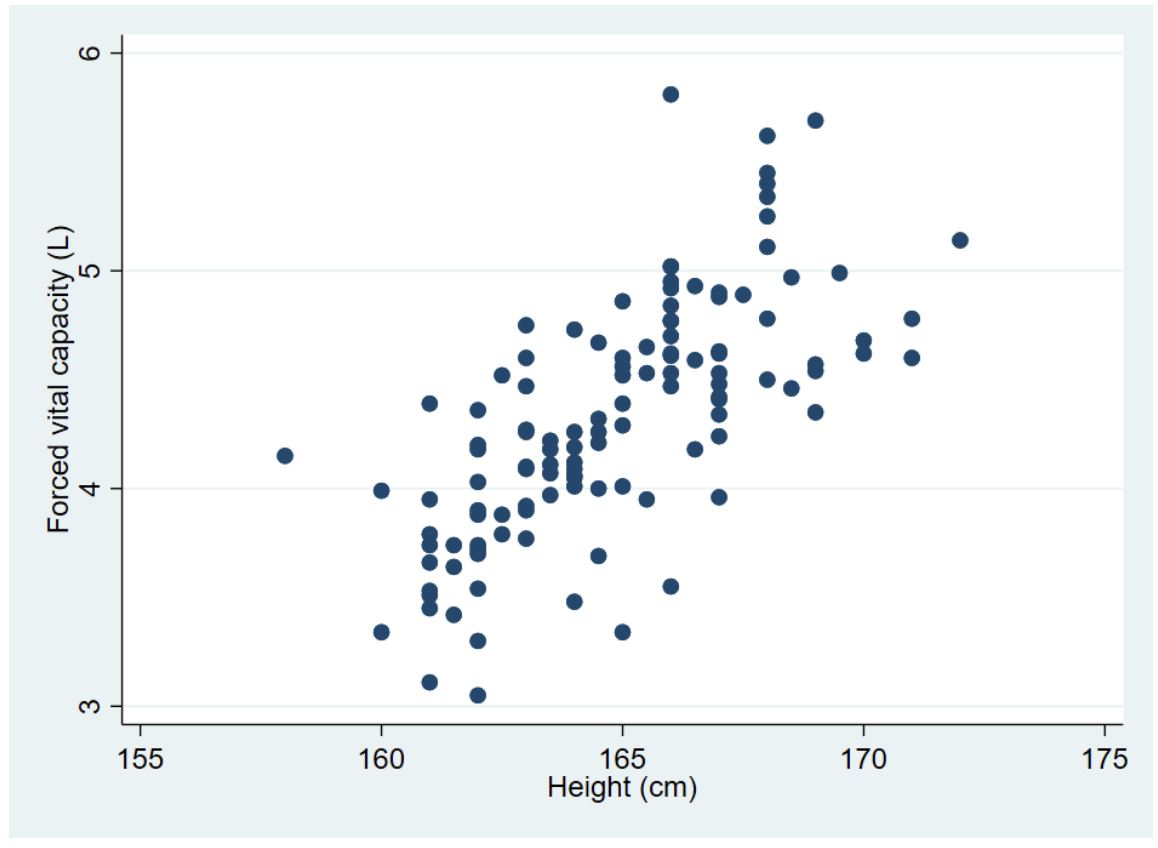
\includegraphics[width=0.66\linewidth]{img/mod08/scatterpng} \caption{Association between height and lung function in 120 adults}\label{fig:scatter-plot}
\end{figure}

\hypertarget{correlation-coefficients}{%
\subsection{Correlation coefficients}\label{correlation-coefficients}}

A correlation coefficient (r) describes how closely the variables are related, that is the strength of linear association between two continuous variables. The range of the coefficient is from +1 to −1 where +1 is a perfect positive association, 0 is no association and −1 is a perfect inverse association. In general, an absolute (disregarding the sign) r value below 0.3 indicates a weak association, 0.3 to \textless{} 0.6 is fair association, 0.6 to \textless{} 0.8 is a moderate association, and \(\ge\) 0.8 indicates a strong association.

The coefficient is positive when large values of one variable tend to occur with large values of the other, and small values of one variable (y) tend to occur with small values of the other (x) (Figure \ref{fig:scatter-plot-four} (a and b)). For example, height and weight in healthy children or age and blood pressure.

The coefficient is negative when large values of one variable tend to occur with small values of the other, and small values of one variable tend to occur with large values of the other (Figure \ref{fig:scatter-plot-four} (c and d)). For example, percentage immunised against infectious diseases and under-five mortality rate.

\begin{figure}
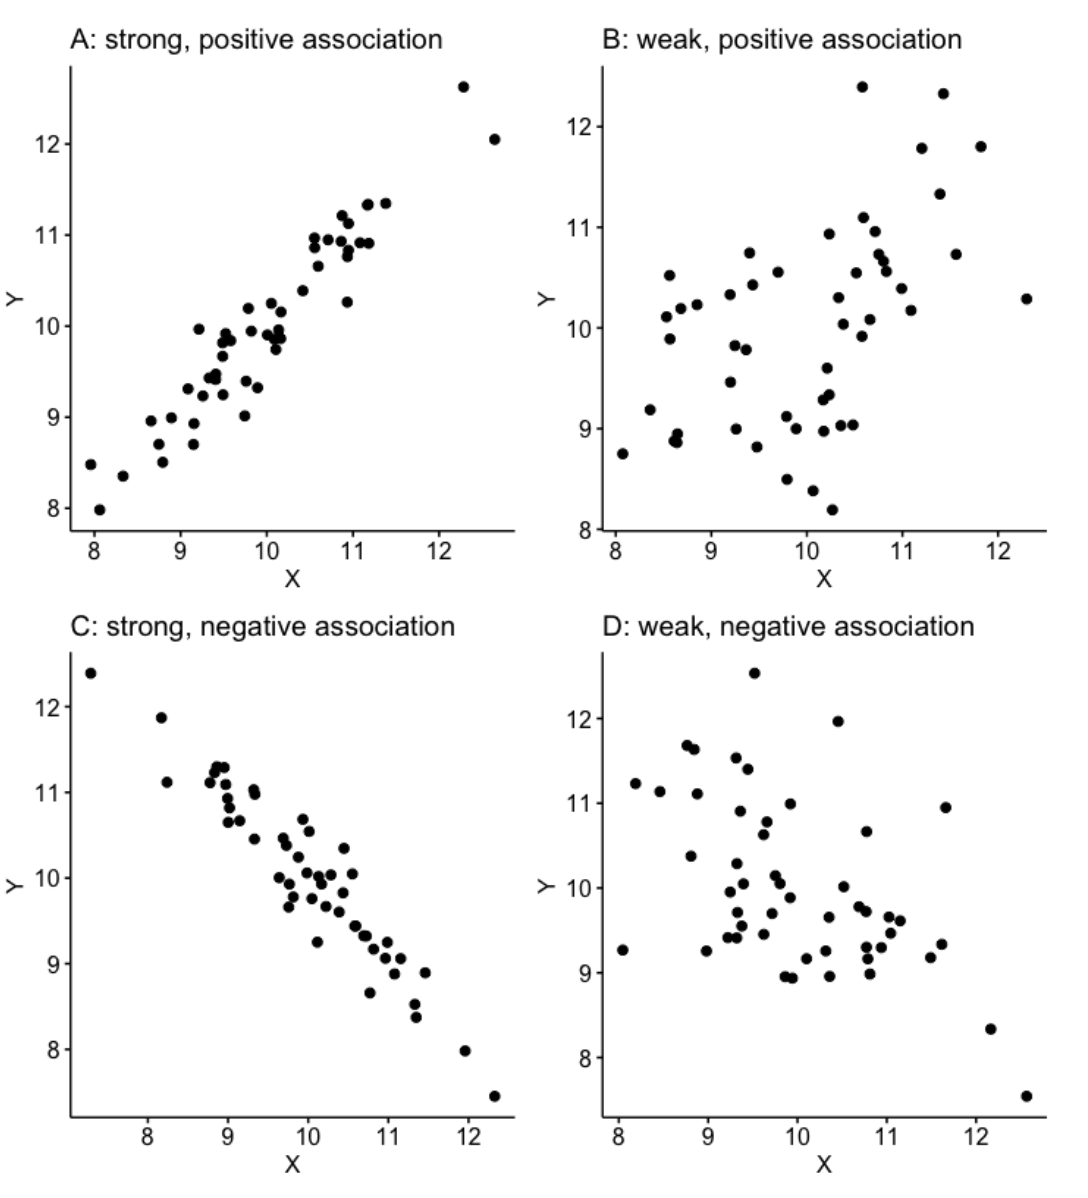
\includegraphics[width=0.66\linewidth]{img/mod08/scatterplot-four-plots} \caption{Scatter plots demonstrating strong and weak, positive and negative associations}\label{fig:scatter-plot-four}
\end{figure}

The P value associated with an r value is an estimate of whether the correlation coefficient is significantly different from zero. However, a correlation coefficient that does not have a significant P value does not imply that there is no relationship because the correlation coefficient only tests for a linear association and there may be a non-linear relationship such as a curved or irregular relationship.

The assumptions for using a Pearson's correlation coefficient are that:

\begin{itemize}
\tightlist
\item
  observations are independent;
\item
  both variables are continuous variables;
\item
  the relationship between the two variables is linear.
\end{itemize}

There is a further assumption that the data follow a bivariate normal distribution. This assumes: \emph{y} follows a normal distribution for given values of \emph{x}; and \emph{x} follows a normal distribution for given values of \emph{y}. This is quite a technical assumption that we do not discuss further.

There are two types of correlation coefficients-- the correct one to use is determined by the nature of the variables as shown in Table \ref{tab:mod08-correlation-coefficients}).

 
  \providecommand{\huxb}[2]{\arrayrulecolor[RGB]{#1}\global\arrayrulewidth=#2pt}
  \providecommand{\huxvb}[2]{\color[RGB]{#1}\vrule width #2pt}
  \providecommand{\huxtpad}[1]{\rule{0pt}{#1}}
  \providecommand{\huxbpad}[1]{\rule[-#1]{0pt}{#1}}

\begin{table}[ht]
\begin{centerbox}
\begin{threeparttable}
\captionsetup{justification=centering,singlelinecheck=off}
\caption{\label{tab:mod08-correlation-coefficients} Correlation coefficients and their application}
 \setlength{\tabcolsep}{0pt}
\begin{tabularx}{0.95\textwidth}{p{0.475\textwidth} p{0.475\textwidth}}


\hhline{>{\huxb{0, 0, 0}{0.4}}->{\huxb{0, 0, 0}{0.4}}-}
\arrayrulecolor{black}

\multicolumn{1}{!{\huxvb{0, 0, 0}{0}}p{0.475\textwidth}!{\huxvb{0, 0, 0}{0}}}{\hspace{0pt}\parbox[b]{0.475\textwidth-0pt-6pt}{\huxtpad{6pt + 1em}\raggedright \textbf{Correlation coefficient}\huxbpad{6pt}}} &
\multicolumn{1}{p{0.475\textwidth}!{\huxvb{0, 0, 0}{0}}}{\hspace{6pt}\parbox[b]{0.475\textwidth-6pt-0pt}{\huxtpad{6pt + 1em}\raggedright \textbf{Application}\huxbpad{6pt}}} \tabularnewline[-0.5pt]


\hhline{>{\huxb{0, 0, 0}{0.4}}->{\huxb{0, 0, 0}{0.4}}-}
\arrayrulecolor{black}

\multicolumn{1}{!{\huxvb{0, 0, 0}{0}}p{0.475\textwidth}!{\huxvb{0, 0, 0}{0}}}{\hspace{0pt}\parbox[b]{0.475\textwidth-0pt-6pt}{\huxtpad{6pt + 1em}\raggedright Pearson’s correlation coefficient: r\huxbpad{6pt}}} &
\multicolumn{1}{p{0.475\textwidth}!{\huxvb{0, 0, 0}{0}}}{\hspace{6pt}\parbox[b]{0.475\textwidth-6pt-0pt}{\huxtpad{6pt + 1em}\raggedright Both variables are continuous and a bivariate normal distribution can be assumed\huxbpad{6pt}}} \tabularnewline[-0.5pt]


\hhline{}
\arrayrulecolor{black}

\multicolumn{1}{!{\huxvb{0, 0, 0}{0}}p{0.475\textwidth}!{\huxvb{0, 0, 0}{0}}}{\hspace{0pt}\parbox[b]{0.475\textwidth-0pt-6pt}{\huxtpad{6pt + 1em}\raggedright Spearman’s rank correlation: rho\huxbpad{6pt}}} &
\multicolumn{1}{p{0.475\textwidth}!{\huxvb{0, 0, 0}{0}}}{\hspace{6pt}\parbox[b]{0.475\textwidth-6pt-0pt}{\huxtpad{6pt + 1em}\raggedright Bivariate normality cannot be assumed. Also useful when at least one of the variables is ordinal\huxbpad{6pt}}} \tabularnewline[-0.5pt]


\hhline{>{\huxb{0, 0, 0}{0.4}}->{\huxb{0, 0, 0}{0.4}}-}
\arrayrulecolor{black}
\end{tabularx}
\end{threeparttable}\par\end{centerbox}

\end{table}
 

Spearman's \(\rho\) is calculated using the ranks of the data, rather than the actual values of the data. We will see further examples of such methods in Module 9, when we consider non-parametric tests, which are often based on ranks.

Correlation coefficients are often presented in the form of a \emph{correlation matrix} which can display the correlation between a number of variables in a single table (Table \ref{tab:corrmatrix}).

\begin{longtable}[]{@{}
  >{\raggedright\arraybackslash}p{(\columnwidth - 4\tabcolsep) * \real{0.1806}}
  >{\raggedright\arraybackslash}p{(\columnwidth - 4\tabcolsep) * \real{0.1944}}
  >{\raggedright\arraybackslash}p{(\columnwidth - 4\tabcolsep) * \real{0.1944}}@{}}
\caption{\label{tab:corrmatrix} Correlation matrix for Height and FVC}\tabularnewline
\toprule()
\endhead
& Height & FVC \\
Height & 1 & \begin{minipage}[t]{\linewidth}\raggedright
0.70\\
P \textless{} 0.0001\strut
\end{minipage} \\
FVC & \begin{minipage}[t]{\linewidth}\raggedright
0.70\\
P \textless{} 0.0001\strut
\end{minipage} & 1 \\
\bottomrule()
\end{longtable}

This correlation matrix shows that the Pearson's correlation coefficient between height and lung function is 0.70 with P\textless0.0001 indicating very strong evidence of a linear association between height and FVC. A correlation matrix sometimes includes correlations between the same variable, indicated as a correlation coefficient of 1. For example, \(Height\) is perfectly correlated with itself (i.e.~has a correlation coefficient of 1). Similarly, \(FVC\) is perfectly correlated with itself.

This r value was calculated for the full data set of 120 adults who had heights ranging from 160 to 172cms. If the r value is calculated for the 60 adults with a height less than 165cms, it is much lower at 0.433 although significant at P=0.001. In general, r values are higher for a wider range of values on the x axis even though the relationship between the two variables remains the same.

Correlation coefficients are rarely used as important statistics in their own right because they do not fully explain the relationship between the two variables and the range of the data has an important influence on the size of the coefficient. In addition, the statistical significance of the correlation coefficient is often over interpreted because a small correlation which is of no clinical importance can become statistically significant even with a relatively small sample size. For example, a poor correlation of 0.3 will be statistically significant if the sample size is large enough.

\hypertarget{linear-regression}{%
\section{Linear regression}\label{linear-regression}}

The nature of a relationship between two variables is more fully described using regression. There are two principal purposes for building a regression model. The most common is to build a predictive model, for example in situations in which age and gender are used to predict normal values of characteristics such as lung size or body mass index. Normal values are the range of values that occur naturally in the general population.

The second purpose for using a regression model is for testing the hypothesis that there is a linear relationship between one or more explanatory variables and an outcome variable. For example, a regression model can be used to test the extent to which age predicts BMI or to test the hypothesis that two groups with a different dietary regime have significantly different BMI values after adjusting for age differences.

From Worked Example 8.1, we can be also plot a regression line through the scatter. Figure \ref{fig:scatter-plot-line} shows the data overlayed with the fitted regression line.

\begin{figure}
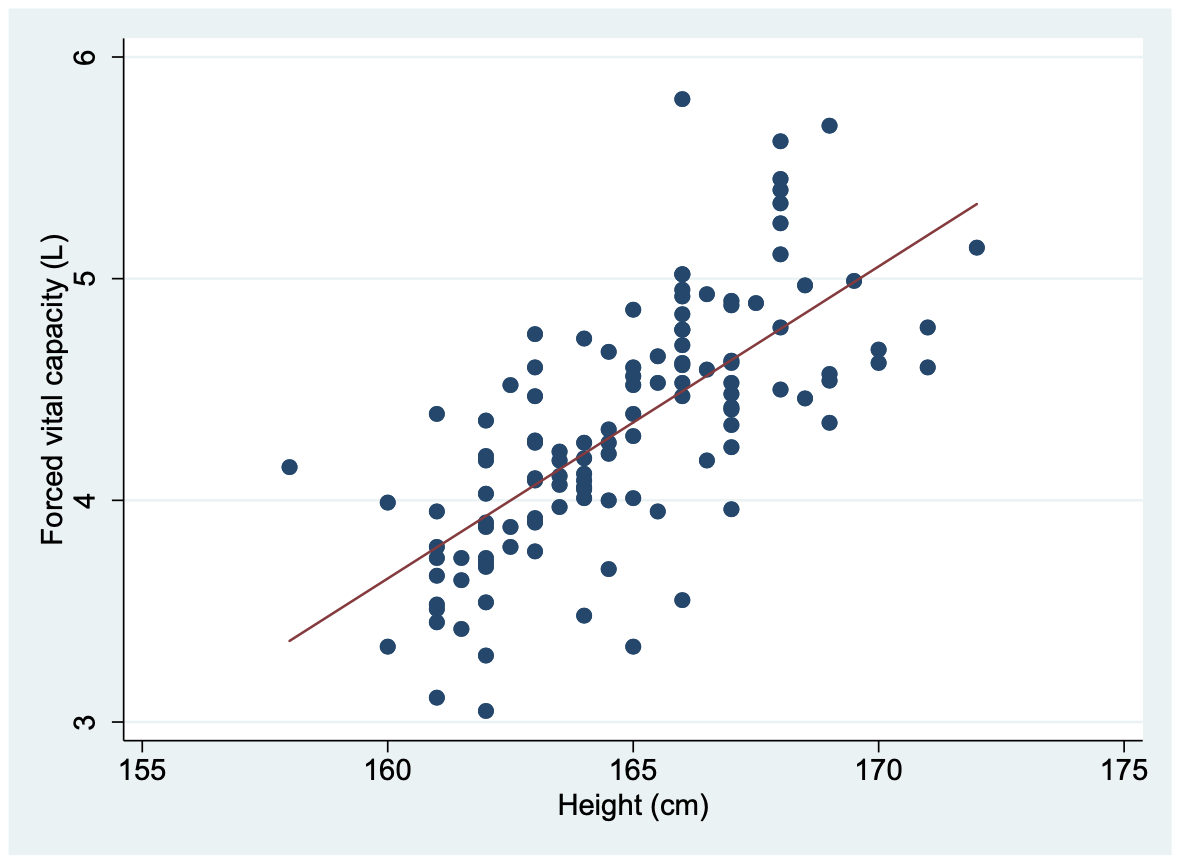
\includegraphics[width=0.66\linewidth]{img/mod08/scatterplot-line-fvc-height} \caption{Association between height and lung function in 120 adults}\label{fig:scatter-plot-line}
\end{figure}

The line through the plot is called the line of `best fit' because the size of the deviations between the data points and the line is minimised in the calculation. The distance between each data point and the regression line is called a `residual'.

\hypertarget{regression-equations}{%
\subsection{Regression equations}\label{regression-equations}}

The mathematical equation for the line explains the relationship between the two variables. The equation of the regression line is as follows:

\[y = \beta_{0} + \beta_{1}x\]

This line is shown in Figure \ref{fig:regression-parameters} using the notation shown in Table \ref{tab:regression-notation}.

\begin{figure}
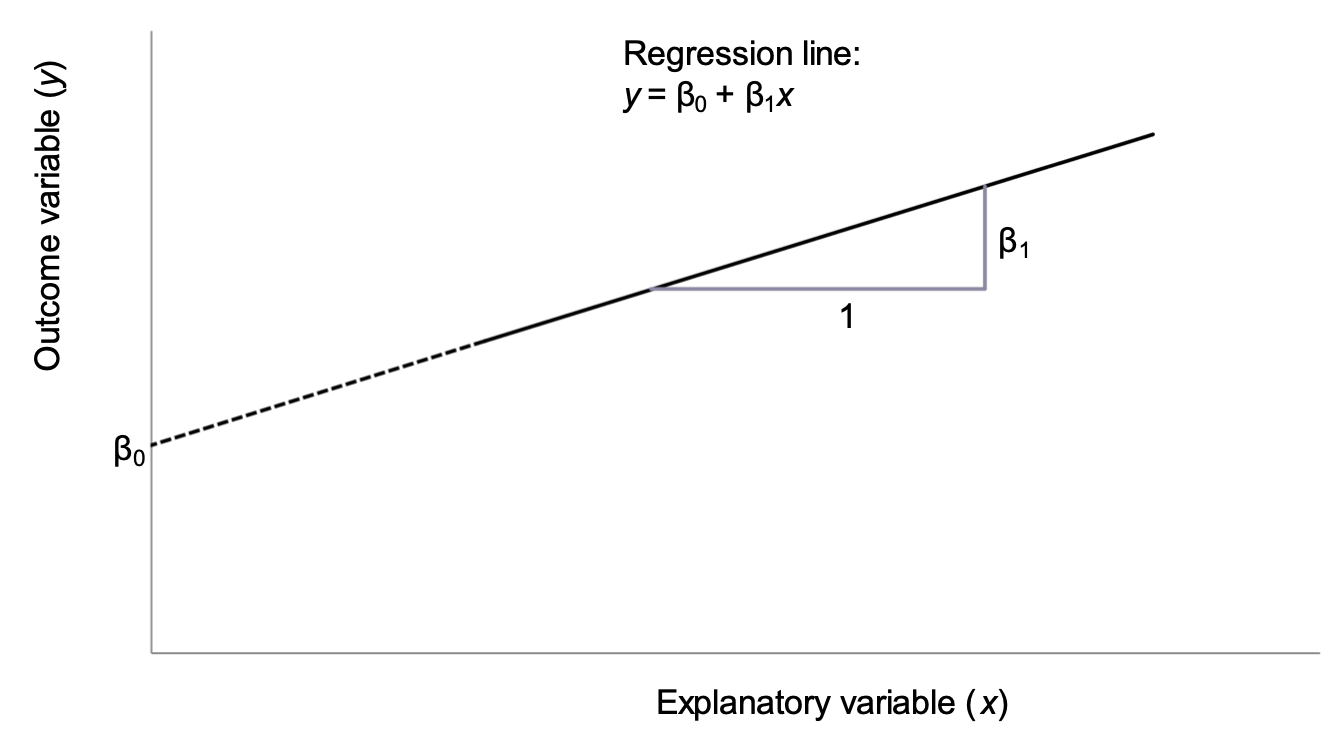
\includegraphics[width=0.66\linewidth]{img/mod08/regression-line-parameters} \caption{Coefficients of a linear regression equation}\label{fig:regression-parameters}
\end{figure}

 
  \providecommand{\huxb}[2]{\arrayrulecolor[RGB]{#1}\global\arrayrulewidth=#2pt}
  \providecommand{\huxvb}[2]{\color[RGB]{#1}\vrule width #2pt}
  \providecommand{\huxtpad}[1]{\rule{0pt}{#1}}
  \providecommand{\huxbpad}[1]{\rule[-#1]{0pt}{#1}}

\begin{table}[ht]
\begin{centerbox}
\begin{threeparttable}
\captionsetup{justification=centering,singlelinecheck=off}
\caption{\label{tab:regression-notation} Notation for linear regression equation}
 \setlength{\tabcolsep}{0pt}
\begin{tabularx}{0.8\textwidth}{p{0.4\textwidth} p{0.4\textwidth}}


\hhline{>{\huxb{0, 0, 0}{0.4}}->{\huxb{0, 0, 0}{0.4}}-}
\arrayrulecolor{black}

\multicolumn{1}{!{\huxvb{0, 0, 0}{0}}p{0.4\textwidth}!{\huxvb{0, 0, 0}{0}}}{\hspace{0pt}\parbox[b]{0.4\textwidth-0pt-6pt}{\huxtpad{6pt + 1em}\raggedright \textbf{Symbol}\huxbpad{6pt}}} &
\multicolumn{1}{p{0.4\textwidth}!{\huxvb{0, 0, 0}{0}}}{\hspace{6pt}\parbox[b]{0.4\textwidth-6pt-0pt}{\huxtpad{6pt + 1em}\raggedright \textbf{Interpretation}\huxbpad{6pt}}} \tabularnewline[-0.5pt]


\hhline{>{\huxb{0, 0, 0}{0.4}}->{\huxb{0, 0, 0}{0.4}}-}
\arrayrulecolor{black}

\multicolumn{1}{!{\huxvb{0, 0, 0}{0}}p{0.4\textwidth}!{\huxvb{0, 0, 0}{0}}}{\hspace{0pt}\parbox[b]{0.4\textwidth-0pt-6pt}{\huxtpad{6pt + 1em}\raggedright y\huxbpad{6pt}}} &
\multicolumn{1}{p{0.4\textwidth}!{\huxvb{0, 0, 0}{0}}}{\hspace{6pt}\parbox[b]{0.4\textwidth-6pt-0pt}{\huxtpad{6pt + 1em}\raggedright Observed value of the outcome variable\huxbpad{6pt}}} \tabularnewline[-0.5pt]


\hhline{}
\arrayrulecolor{black}

\multicolumn{1}{!{\huxvb{0, 0, 0}{0}}p{0.4\textwidth}!{\huxvb{0, 0, 0}{0}}}{\hspace{0pt}\parbox[b]{0.4\textwidth-0pt-6pt}{\huxtpad{6pt + 1em}\raggedright x\huxbpad{6pt}}} &
\multicolumn{1}{p{0.4\textwidth}!{\huxvb{0, 0, 0}{0}}}{\hspace{6pt}\parbox[b]{0.4\textwidth-6pt-0pt}{\huxtpad{6pt + 1em}\raggedright Observed value of the explanatory variable\huxbpad{6pt}}} \tabularnewline[-0.5pt]


\hhline{}
\arrayrulecolor{black}

\multicolumn{1}{!{\huxvb{0, 0, 0}{0}}p{0.4\textwidth}!{\huxvb{0, 0, 0}{0}}}{\hspace{0pt}\parbox[b]{0.4\textwidth-0pt-6pt}{\huxtpad{6pt + 1em}\raggedright β\_0\huxbpad{6pt}}} &
\multicolumn{1}{p{0.4\textwidth}!{\huxvb{0, 0, 0}{0}}}{\hspace{6pt}\parbox[b]{0.4\textwidth-6pt-0pt}{\huxtpad{6pt + 1em}\raggedright Intercept of the regression line\huxbpad{6pt}}} \tabularnewline[-0.5pt]


\hhline{}
\arrayrulecolor{black}

\multicolumn{1}{!{\huxvb{0, 0, 0}{0}}p{0.4\textwidth}!{\huxvb{0, 0, 0}{0}}}{\hspace{0pt}\parbox[b]{0.4\textwidth-0pt-6pt}{\huxtpad{6pt + 1em}\raggedright β\_1\huxbpad{6pt}}} &
\multicolumn{1}{p{0.4\textwidth}!{\huxvb{0, 0, 0}{0}}}{\hspace{6pt}\parbox[b]{0.4\textwidth-6pt-0pt}{\huxtpad{6pt + 1em}\raggedright Slope of the regression line\huxbpad{6pt}}} \tabularnewline[-0.5pt]


\hhline{>{\huxb{0, 0, 0}{0.4}}->{\huxb{0, 0, 0}{0.4}}-}
\arrayrulecolor{black}
\end{tabularx}
\end{threeparttable}\par\end{centerbox}

\end{table}
 

The intercept is the point at which the regression line intersects with the y-axis when the value of `x' is zero. In most cases, the intercept does not have a biologically meaningful interpretation as the explanatory variable cannot take a value of zero. In our working example, the intercept is not meaningful as it is not possible for an adult to have a height of 0cm.

The slope of the line is the predicted change in the outcome variable `y' as the explanatory explanatory variable `x' increases by 1 unit.

An important concept is that regression predicts an expected value of `y' given an observed value of `x': any error around the explanatory variable is not taken into account. For this reason, measurements that can be taken accurately, such as age and height, make good explanatory variables.

\hypertarget{regression-coefficients-estimation}{%
\section{Regression coefficients: estimation}\label{regression-coefficients-estimation}}

Software is always used to estimate the regression equation for a set of data, using the \emph{method of least squares}. This method estimates the intercept and the slope, and also their variability (i.e.~standard errors).

\hypertarget{regression-coefficients-inference}{%
\section{Regression coefficients: inference}\label{regression-coefficients-inference}}

We can use the estimated regression coefficients and their variability to calculate 95\% confidence intervals. Here, a t-value from a t-distribution with \[n - 2\] degrees of freedom is used:

b0 plus/minus t\_n-2 * SE(b0) \emph{
b1 plus/minus t\_n-2 } SE(b1)

Note that as the constant (b0) is not often biologically plausible, the 95\% confidence interval for the constant is often not reported.

The significance of the estimated slope (and less commonly, intercept) can be tested using a t-test. The null hypotheses and the alternative hypothesis for testing the slope of a simple linear regression model are:

H0: beta\_1 = 0
H1: beta\_1 NE 0

To test the null hypothesis for the regression coefficient beta\_1, the following t-test is used:

t = beta\_1 /SE(beta\_1)

This will give a t statistic with an underlying t distribution with n − 2 degrees of freedom, with a corresponding P-value.

Table X.X shows the estimated regression coefficients for our working example.

 
  \providecommand{\huxb}[2]{\arrayrulecolor[RGB]{#1}\global\arrayrulewidth=#2pt}
  \providecommand{\huxvb}[2]{\color[RGB]{#1}\vrule width #2pt}
  \providecommand{\huxtpad}[1]{\rule{0pt}{#1}}
  \providecommand{\huxbpad}[1]{\rule[-#1]{0pt}{#1}}

\begin{table}[ht]
\begin{centerbox}
\begin{threeparttable}
\captionsetup{justification=centering,singlelinecheck=off}
\caption{\label{tab:estimated-regression} Estimated regression coefficients}
 \setlength{\tabcolsep}{0pt}
\begin{tabular}{l l l l l l}


\hhline{>{\huxb{0, 0, 0}{0.4}}->{\huxb{0, 0, 0}{0.4}}->{\huxb{0, 0, 0}{0.4}}->{\huxb{0, 0, 0}{0.4}}->{\huxb{0, 0, 0}{0.4}}->{\huxb{0, 0, 0}{0.4}}-}
\arrayrulecolor{black}

\multicolumn{1}{!{\huxvb{0, 0, 0}{0}}l!{\huxvb{0, 0, 0}{0}}}{\huxtpad{6pt + 1em}\raggedright \hspace{0pt} \textbf{Term} \hspace{6pt}\huxbpad{6pt}} &
\multicolumn{1}{r!{\huxvb{0, 0, 0}{0}}}{\huxtpad{6pt + 1em}\raggedleft \hspace{6pt} \textbf{Estimate} \hspace{6pt}\huxbpad{6pt}} &
\multicolumn{1}{r!{\huxvb{0, 0, 0}{0}}}{\huxtpad{6pt + 1em}\raggedleft \hspace{6pt} \textbf{Standard error} \hspace{6pt}\huxbpad{6pt}} &
\multicolumn{1}{l!{\huxvb{0, 0, 0}{0}}}{\huxtpad{6pt + 1em}\raggedright \hspace{6pt} \textbf{t value} \hspace{6pt}\huxbpad{6pt}} &
\multicolumn{1}{l!{\huxvb{0, 0, 0}{0}}}{\huxtpad{6pt + 1em}\raggedright \hspace{6pt} \textbf{P value} \hspace{6pt}\huxbpad{6pt}} &
\multicolumn{1}{l!{\huxvb{0, 0, 0}{0}}}{\huxtpad{6pt + 1em}\raggedright \hspace{6pt} \textbf{95\% Confidence interval} \hspace{0pt}\huxbpad{6pt}} \tabularnewline[-0.5pt]


\hhline{>{\huxb{0, 0, 0}{0.4}}->{\huxb{0, 0, 0}{0.4}}->{\huxb{0, 0, 0}{0.4}}->{\huxb{0, 0, 0}{0.4}}->{\huxb{0, 0, 0}{0.4}}->{\huxb{0, 0, 0}{0.4}}-}
\arrayrulecolor{black}

\multicolumn{1}{!{\huxvb{0, 0, 0}{0}}l!{\huxvb{0, 0, 0}{0}}}{\huxtpad{6pt + 1em}\raggedright \hspace{0pt} Intercept \hspace{6pt}\huxbpad{6pt}} &
\multicolumn{1}{r!{\huxvb{0, 0, 0}{0}}}{\huxtpad{6pt + 1em}\raggedleft \hspace{6pt} -18.9\hphantom{0} \hspace{6pt}\huxbpad{6pt}} &
\multicolumn{1}{r!{\huxvb{0, 0, 0}{0}}}{\huxtpad{6pt + 1em}\raggedleft \hspace{6pt} 2.19\hphantom{0} \hspace{6pt}\huxbpad{6pt}} &
\multicolumn{1}{l!{\huxvb{0, 0, 0}{0}}}{\huxtpad{6pt + 1em}\raggedright \hspace{6pt} t=-8.60, 118df \hspace{6pt}\huxbpad{6pt}} &
\multicolumn{1}{l!{\huxvb{0, 0, 0}{0}}}{\huxtpad{6pt + 1em}\raggedright \hspace{6pt} $<$0.001 \hspace{6pt}\huxbpad{6pt}} &
\multicolumn{1}{l!{\huxvb{0, 0, 0}{0}}}{\huxtpad{6pt + 1em}\raggedright \hspace{6pt} -23.22 to -14.53 \hspace{0pt}\huxbpad{6pt}} \tabularnewline[-0.5pt]


\hhline{}
\arrayrulecolor{black}

\multicolumn{1}{!{\huxvb{0, 0, 0}{0}}l!{\huxvb{0, 0, 0}{0}}}{\huxtpad{6pt + 1em}\raggedright \hspace{0pt} Height \hspace{6pt}\huxbpad{6pt}} &
\multicolumn{1}{r!{\huxvb{0, 0, 0}{0}}}{\huxtpad{6pt + 1em}\raggedleft \hspace{6pt} 0.14 \hspace{6pt}\huxbpad{6pt}} &
\multicolumn{1}{r!{\huxvb{0, 0, 0}{0}}}{\huxtpad{6pt + 1em}\raggedleft \hspace{6pt} 0.013 \hspace{6pt}\huxbpad{6pt}} &
\multicolumn{1}{l!{\huxvb{0, 0, 0}{0}}}{\huxtpad{6pt + 1em}\raggedright \hspace{6pt} t=10.58, 118df \hspace{6pt}\huxbpad{6pt}} &
\multicolumn{1}{l!{\huxvb{0, 0, 0}{0}}}{\huxtpad{6pt + 1em}\raggedright \hspace{6pt} $<$0.001 \hspace{6pt}\huxbpad{6pt}} &
\multicolumn{1}{l!{\huxvb{0, 0, 0}{0}}}{\huxtpad{6pt + 1em}\raggedright \hspace{6pt} 0.11 to 0.17 \hspace{0pt}\huxbpad{6pt}} \tabularnewline[-0.5pt]


\hhline{>{\huxb{0, 0, 0}{0.4}}->{\huxb{0, 0, 0}{0.4}}->{\huxb{0, 0, 0}{0.4}}->{\huxb{0, 0, 0}{0.4}}->{\huxb{0, 0, 0}{0.4}}->{\huxb{0, 0, 0}{0.4}}-}
\arrayrulecolor{black}
\end{tabular}
\end{threeparttable}\par\end{centerbox}

\end{table}
 

From this output, we see that the slope is estimated as 0.141 with an estimated intercept of -18.873. Therefore, the regression equation is estimated as:

FVC (L) = − 18.873 + (0.141 \(\times\) Height in cm)

This equation can be used to predict FVC for a person of a given height. For example, the predicted FVC for a person 165 cm tall is estimated as:

FVC = − 18.87347 + (0.1407567 \(\times\) 165.0) = 4.40 L.

Note that for the purpose of prediction we have kept all the decimal places in the coefficients to avoid rounding error in the intermediate calculation.

From this model, there is very strong evidence of a linear association between FVC and height in cm (P \textless{} 0.001).

\hypertarget{fit-of-a-linear-regression-model}{%
\subsection{Fit of a linear regression model}\label{fit-of-a-linear-regression-model}}

After fitting a linear regression model, it is important to know how well the model fits the observed data. One way of assessing the model fit is to compute a statistic called coefficient of determination, denoted by \(R^2\). It is the square of the Pearson correlation coefficient \(r: r^2 = R^2\). Since the range of \(r\) is from −1 to 1, \(R^2\) must lie between 0 and 1.

\(R^2\) can be interpreted as the proportion of variability in y that can be explained by variability in x. Hence, the following conditions may arise:

If \(R^2 = 1\), then all variation in y can be explained by variation of x and all data points fall on the regression line.

If \(R^2 = 0\), then none of the variation in y is related to x at all, and the variable x explains none of the variability in y.

If \(0 < R^2 <1\), then the variability of y can be partially explained by the variability in x. The larger the \(R^2\) value, the better is the fit of the regression model.

\hypertarget{assumptions-for-linear-regression}{%
\subsection{Assumptions for linear regression}\label{assumptions-for-linear-regression}}

Regression is robust to moderate degrees of non-normality in the variables, provided that the sample size is large enough and that there are no influential outliers. Also, the regression equation describes the relationship between the variables and this is not influenced as much by the spread of the data as the correlation coefficient is.

The assumptions that must be met when using linear regression are as follows:

\begin{itemize}
\tightlist
\item
  observations are independent;
\item
  the relationship between the explanatory and the outcome variable is linear;
\item
  the residuals are normally distributed.
\end{itemize}

A residual is defined as the difference between the observed and predicted outcome from the regression model. If the predicted value of the outcome variable is denoted by \(\hat y\) then:

\[ \text{Residual} = \text{observed} - \text{predicted} = y - \hat y\]

It is important for regression modelling that the data are collected in a period when the relationship remains constant. For example, in building a model to predict normal values for lung function the data must be collected when the participants have been resting and not exercising and people taking bronchodilator medications that influence lung capacity should be excluded. In regression, it is not so important that the variables themselves are normally distributed, but it is important that the residuals are. Scatter plots and specific diagnostic tests can be used to check the regression assumptions. Some of these will not be covered in this introductory course but will be discussed in detail in the \textbf{Advanced Biostatistics} course.

The distribution of the residuals should always be checked. Large residuals can indicate unusual points or points that may exert undue influence on the estimated regression slope.

The histogram of residuals from the model is shown in Figure 8.5. They are normally distributed and indicate that there are no influential outliers so that the assumptions for regression are met.

\begin{figure}
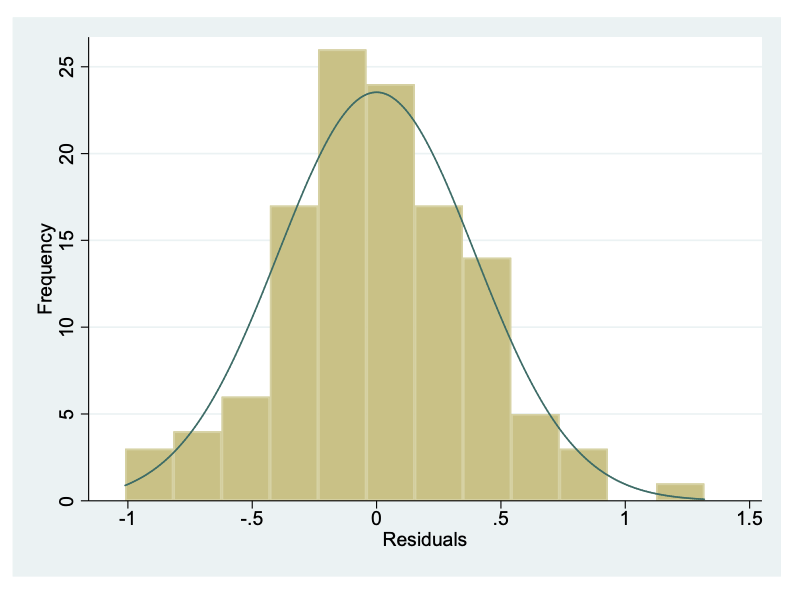
\includegraphics[width=0.66\linewidth]{img/mod08/regression-residual-histogram} \caption{Histogram of regression residuals}\label{fig:residual-hist}
\end{figure}

\hypertarget{critical-appraisal}{%
\subsection{Critical appraisal}\label{critical-appraisal}}

When reading the literature, it is important to be critical about how correlation coefficients are interpreted. It is a good idea to check if a scatter plot is shown to help interpret the relationship and to indicate if there are any influential outliers. Also, question whether the correlation coefficient has been calculated from a random sample and if not, what selected samples the value can be generalised to.

When regression is reported it is essential that the axes are correctly presented so that the equation is predictive. Thus, the explanatory variable must be presented on the x axis and the outcome on the y axis. It is also a good idea to check that all the assumptions are met. Outliers which result in a non-normal distribution of the residuals can severely bias the regression coefficients.

\hypertarget{multiple-linear-regression}{%
\section{Multiple linear regression}\label{multiple-linear-regression}}

In the above example, we have only used a simple linear regression model of two continuous variables. Other more complex models can be built from this e.g.~if we wanted to look at the effect of gender (male vs.~female) as binary indicator in the model while adjusting for the effect of height. In that case we would include both the variables in the model as explanatory variables. In the same way we can include any number of explanatory variables (both continuous and categorical) in the model: this is called a multivariable model. Multivariable models are often used for building predictive equations, for example by using age, height, gender and smoking history to predict lung function, or to adjust for confounding and detect effect modification to investigate the association between an exposure and an outcome factor.

Multiple regression has an important role in investigating causality in epidemiology. The exposure variable under investigation must stay in the model and the effects of other variables which can be confounders or effect-modifiers are tested. The biological, psychological or social meaning of the variables in the model and their interactions are of great importance for interpreting theories of causality.

Other multivariable models include binary logistic regression for use with a binary outcome variable, or Cox regression for survival analyses. These models, together with multiple regression, will be taught in \textbf{PHCM9517: Regression Methods in Biostatistics}.

\hypertarget{stata-notes}{%
\chapter*{\texorpdfstring{\textbf{8} Stata notes}{8 Stata notes}}\label{stata-notes}}
\addcontentsline{toc}{chapter}{\textbf{8} Stata notes}

\hypertarget{creating-a-scatter-plot}{%
\section{Creating a scatter plot}\label{creating-a-scatter-plot}}

We will demonstrate using Stata for correlation and simple linear regression using the dataset \texttt{Example\_8.1.dta}.

To create a scatter plot to explore the association between height and FVC click: \textbf{Graphics \textgreater{} Twoway graph (scatter, line, etc.)}. In the \texttt{twoway} dialog box, click \textbf{Create\ldots{}}

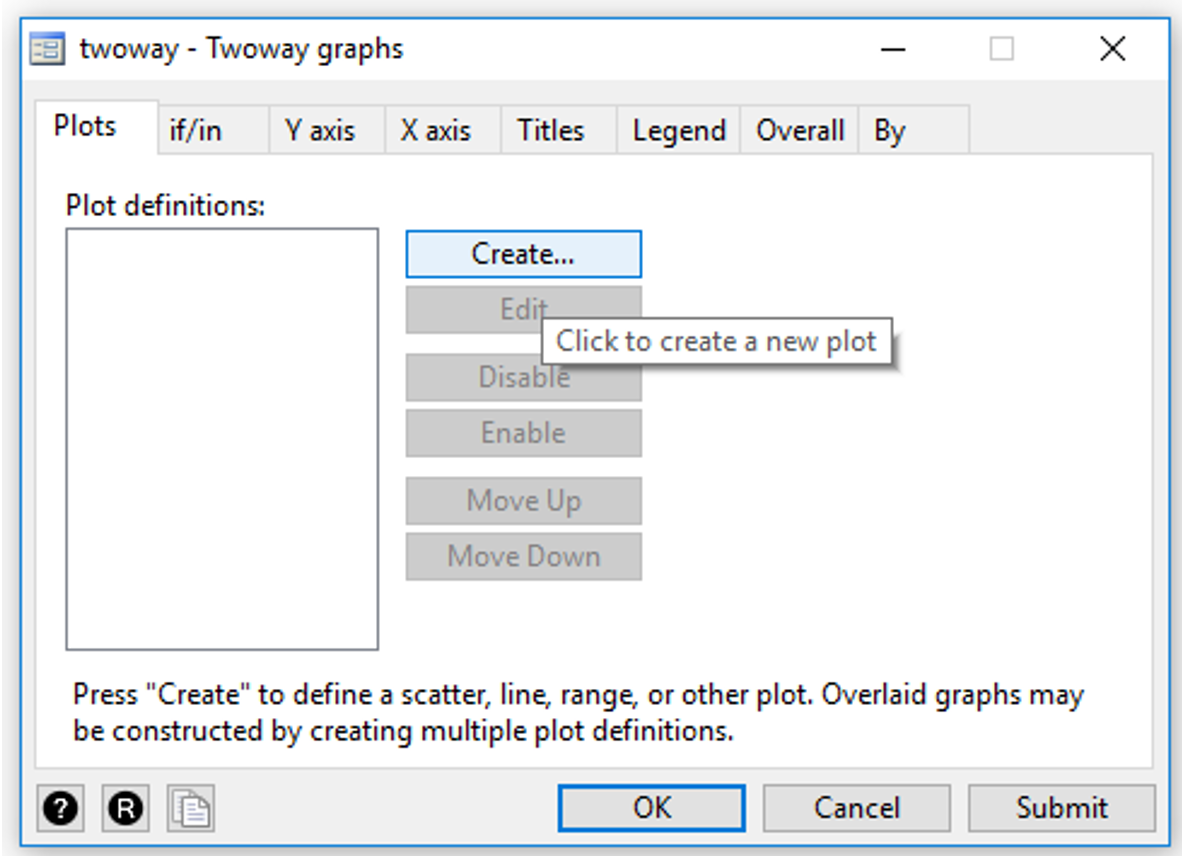
\includegraphics[width=0.66\linewidth]{img/mod08/stata/twoway-1}

A new dialog box will open. Select the \textbf{Basic plots} radio button and highlight \textbf{Scatter} under \textbf{Basic plots: (select type)}. Choose \textbf{FVC} for the \textbf{Y variable} and \textbf{Height} for the \textbf{X variable}.

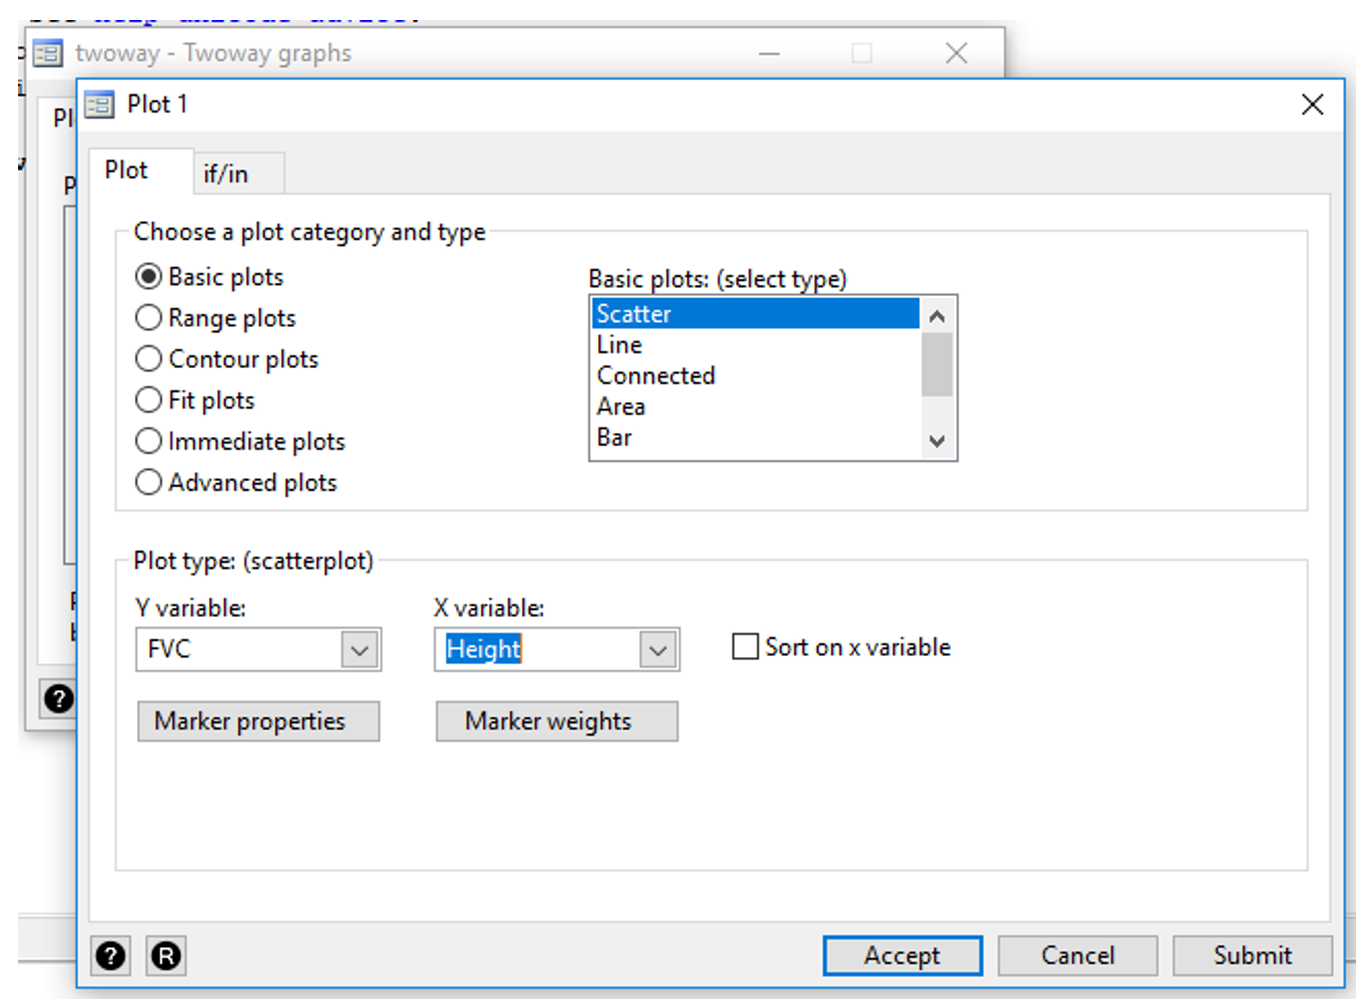
\includegraphics[width=0.66\linewidth]{img/mod08/stata/twoway-2}

Click the \textbf{Accept} button in the \textbf{Plot 1} dialog box to return to the \textbf{twoway} dialog box, then click the \textbf{OK} or \textbf{Submit} button to produce the scatter plot shown in \textbf{Figure 8.1}.

{[}Command: \texttt{twoway\ (scatter\ FVC\ Height)}{]}

To add a fitted line, go back to the \texttt{twoway} dialog box. If you clicked the \textbf{OK} button, you can go to \textbf{Graphics} \textbf{\textgreater{} Twoway} \textbf{graph (scatter, line, etc.)} to bring it back again.

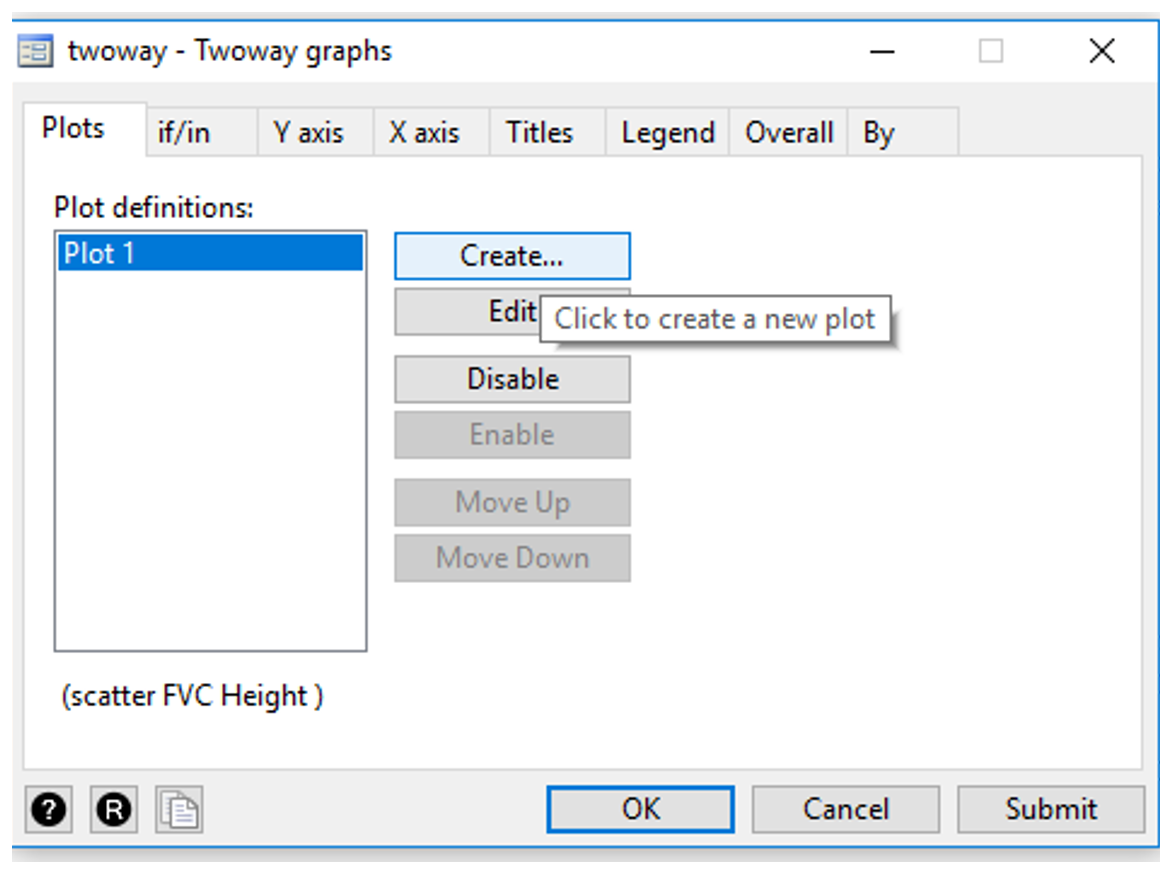
\includegraphics[width=0.66\linewidth]{img/mod08/stata/twoway-3}

Click \textbf{Create\ldots{}}, then select the \textbf{Fit plots} radio button and \textbf{Linear prediction} under \textbf{Fit plots: (select type)}. Choose \textbf{FVC} for the \textbf{Y variable} and \textbf{Height} for the \textbf{X variable}.

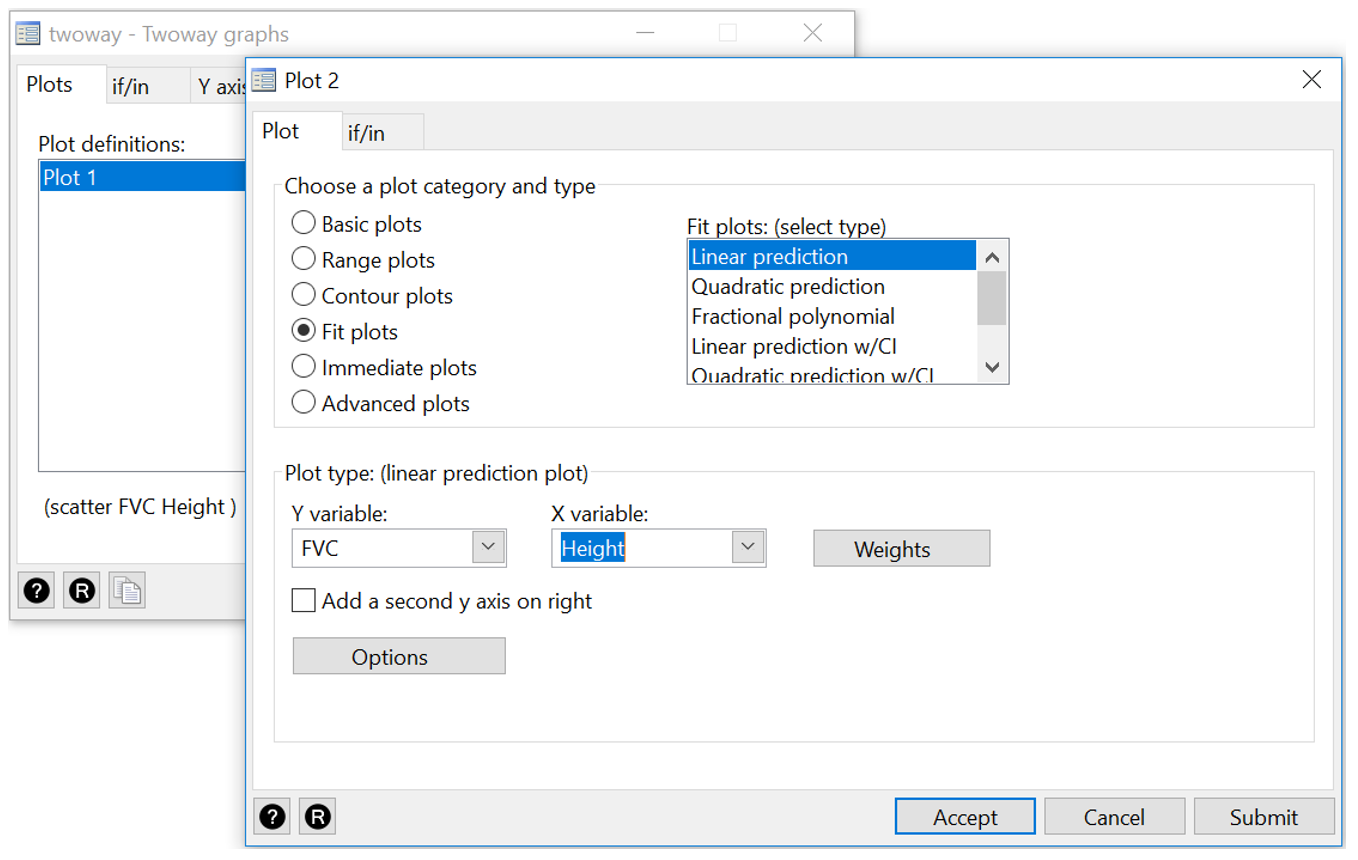
\includegraphics[width=0.66\linewidth]{img/mod08/stata/twoway-4}

Click the \textbf{Accept} button, then the \textbf{OK} or \textbf{Submit} button to produce the scatterplot below.

{[}Command: \texttt{twoway\ (scatter\ FVC\ Height)\ (lfit\ FVC\ Height)}{]}

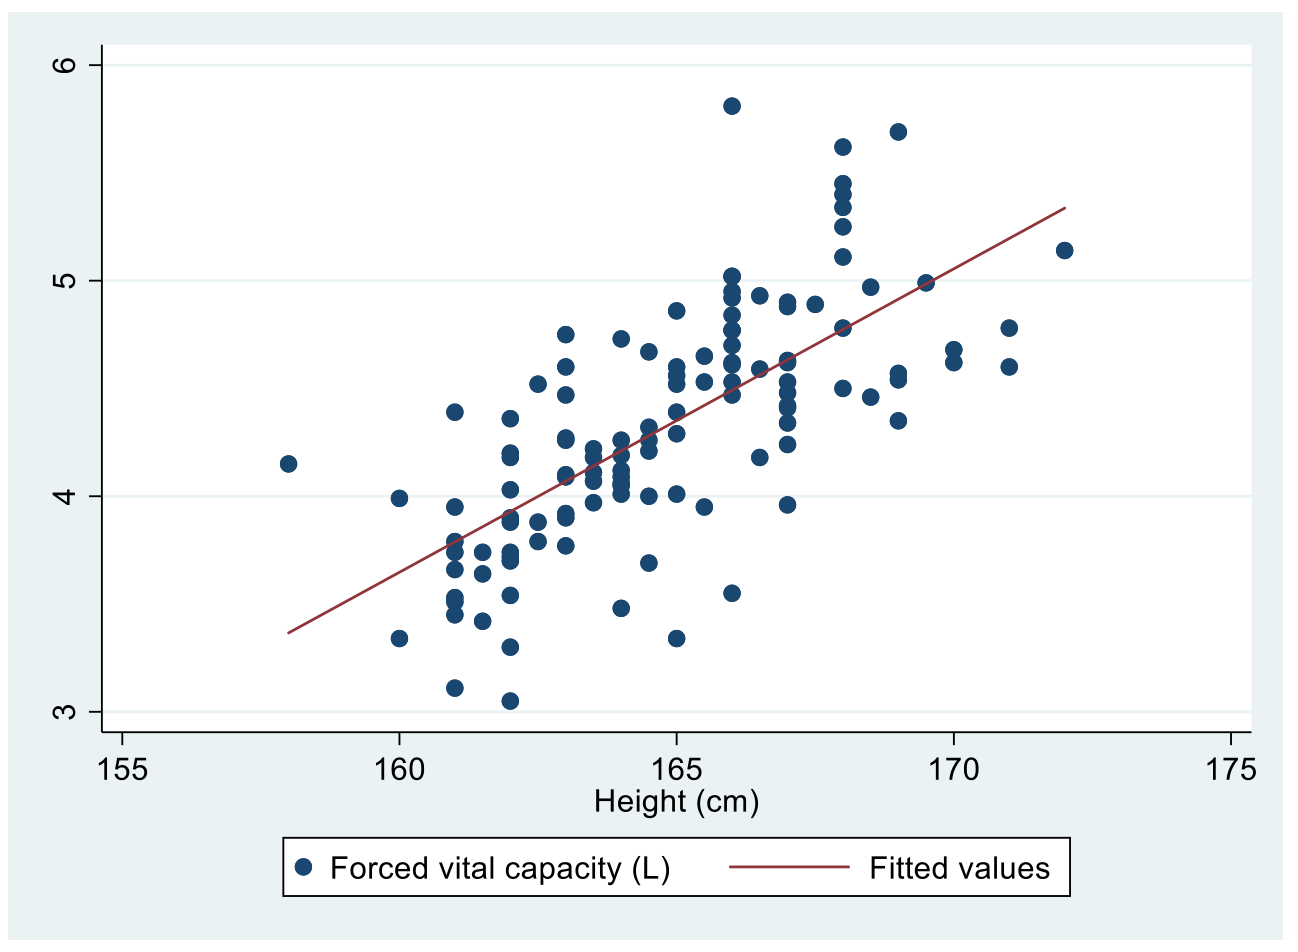
\includegraphics[width=0.66\linewidth]{img/mod08/stata/scatter-1}

Notice that a legend now appears, and the y-axis title is missing. To add a y-axis title, go to the \textbf{Y axis} tab in the \textbf{twoway} dialog box to enter your title as shown below.

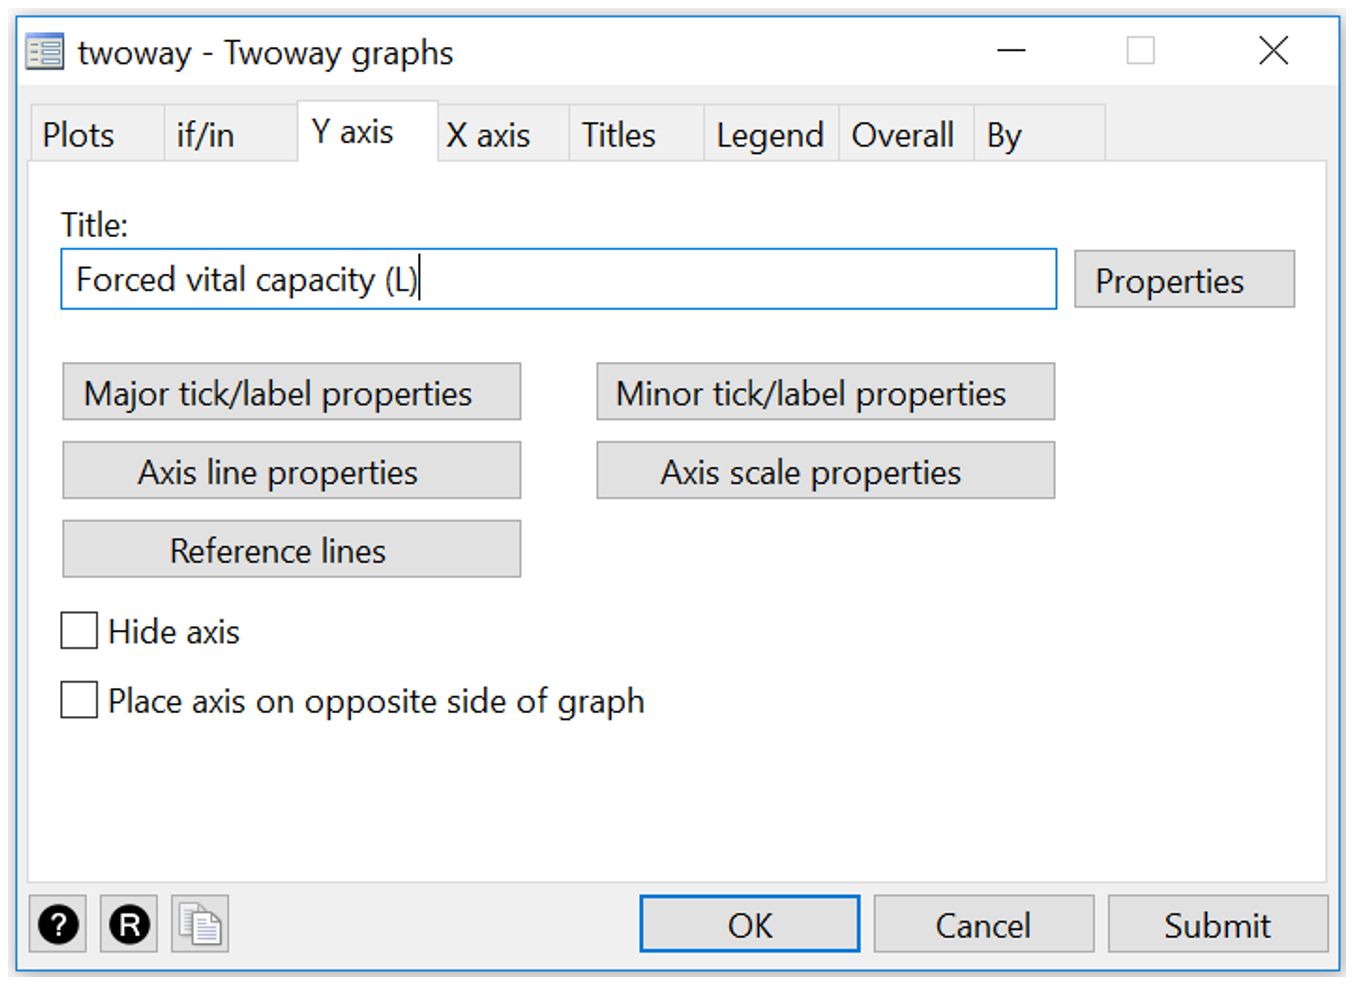
\includegraphics[width=0.66\linewidth]{img/mod08/stata/twoway-5}

You can click the \textbf{Submit} button to check how the scatter plot looks like. Next go the \textbf{Legend} tab and select the \textbf{Hide legend} radio button.

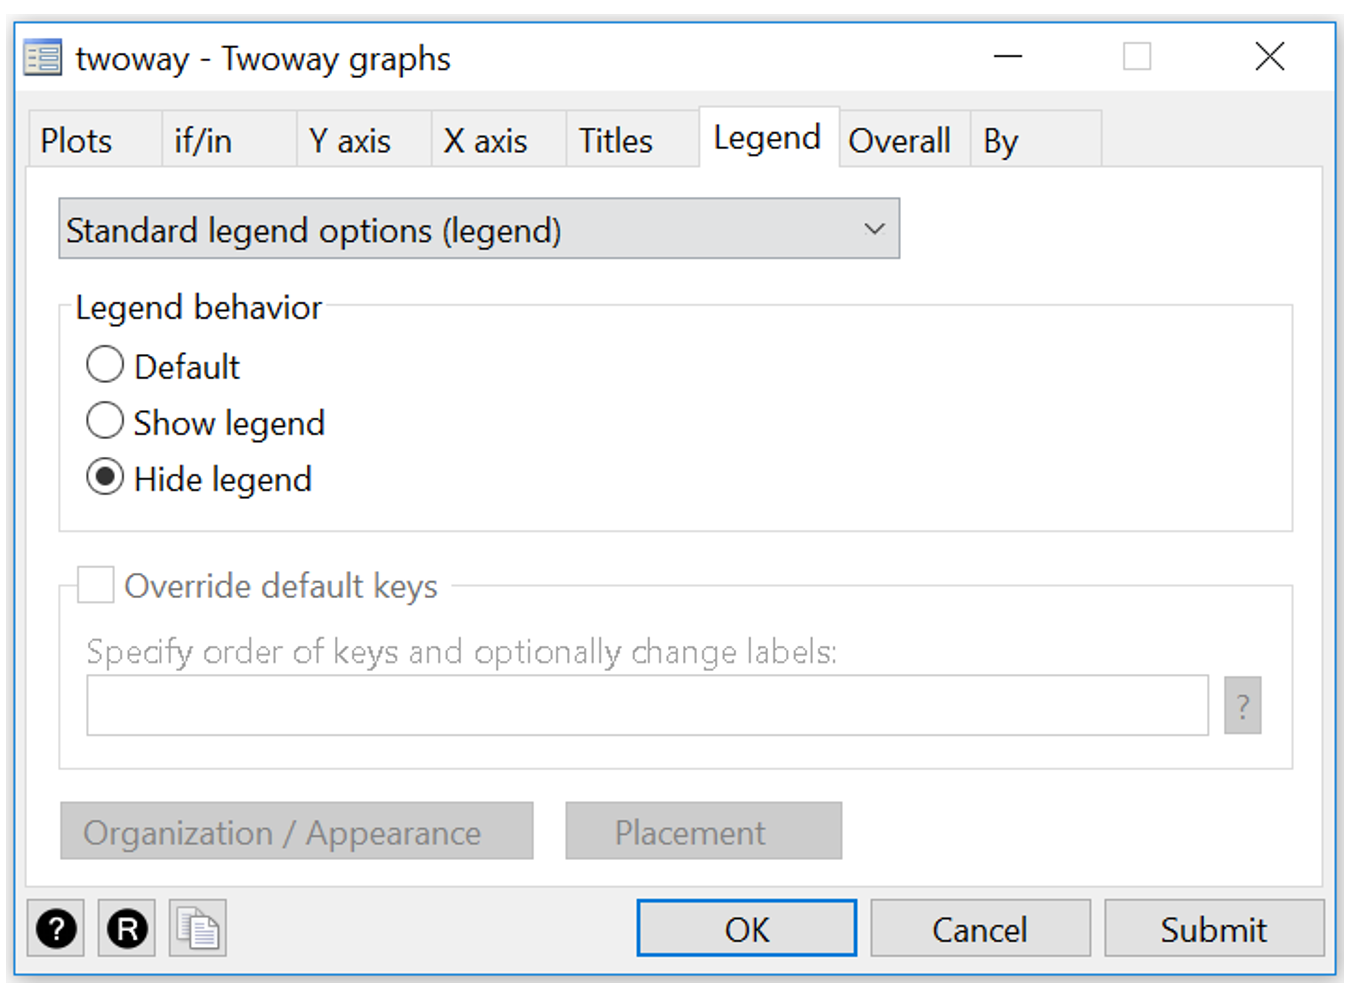
\includegraphics[width=0.66\linewidth]{img/mod08/stata/twoway-6}

Click the \textbf{OK} or \textbf{Submit} button when you are finished to produce \textbf{Figure 8.3}.

{[}Command: \texttt{twoway\ (scatter\ FVC\ Height)\ (lfit\ FVC\ Height),\ ytitle(Forced\ vital\ capacity\ (L))\ legend(off)}{]}

To save your graph, go to \textbf{File \textgreater{} Save} in the \textbf{Graph} window, and be sure to save your file as a PNG file:

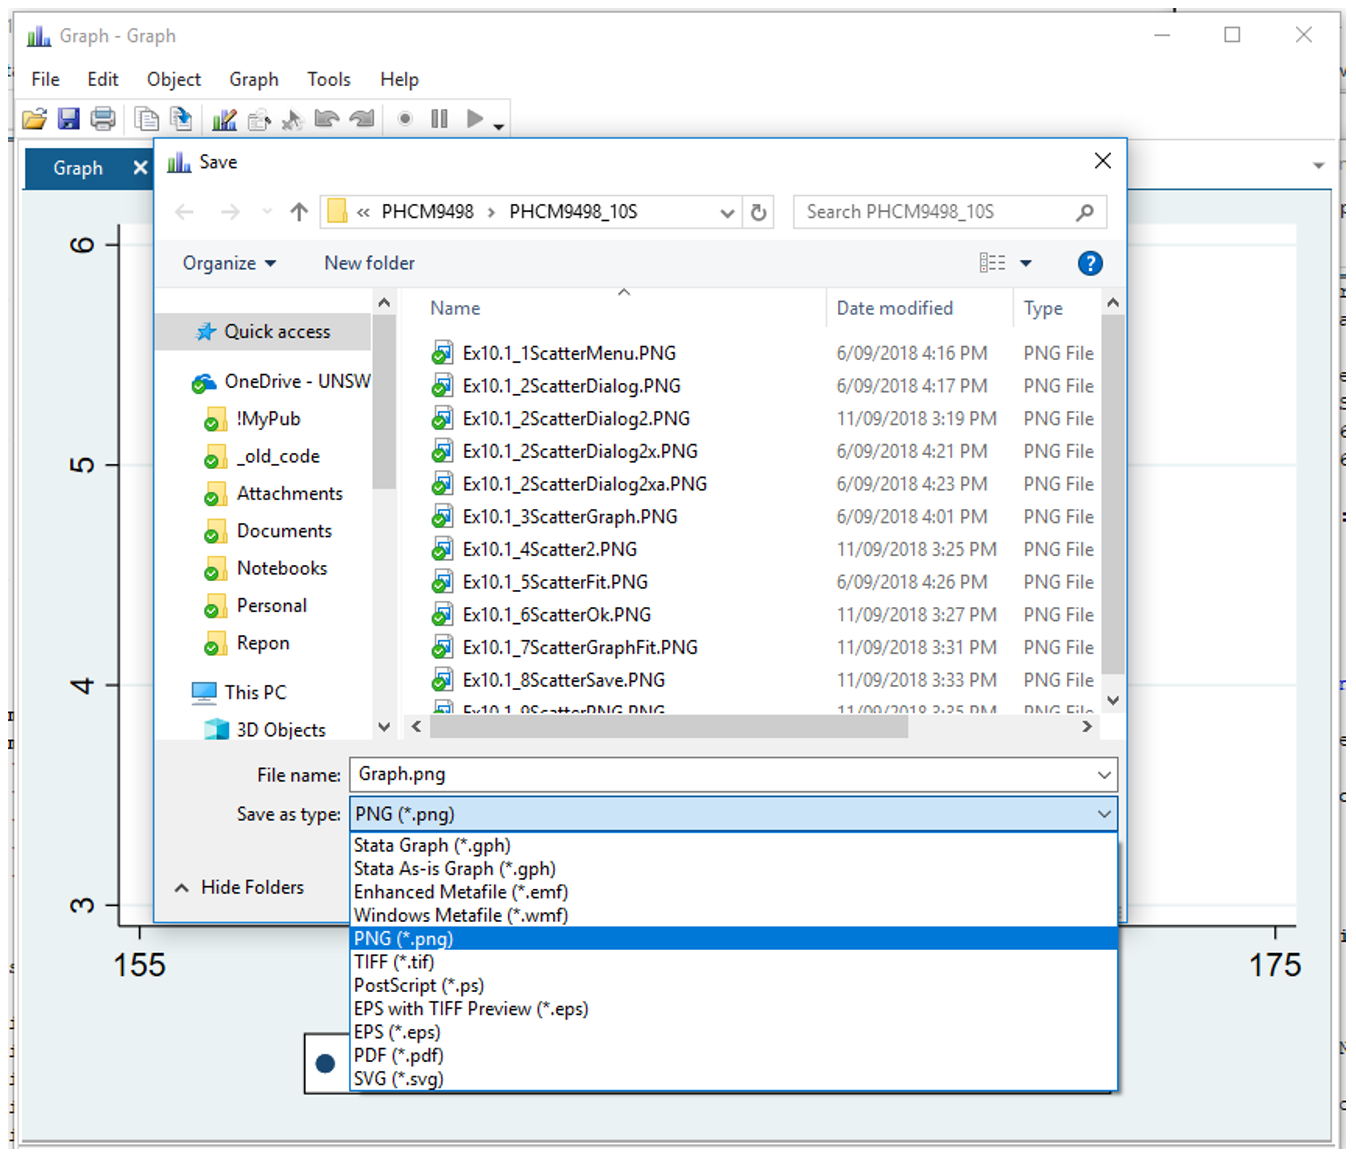
\includegraphics[width=0.66\linewidth]{img/mod08/stata/twoway-7}

\hypertarget{calculating-a-correlation-coefficient}{%
\section{Calculating a correlation coefficient}\label{calculating-a-correlation-coefficient}}

To calculate the Pearson's correlation using the dataset \texttt{Example\_8.1.dta} go to: \textbf{Statistics \textgreater{} Summaries, tables, and tests \textgreater{} Summary and descriptive statistics \textgreater{} Pairwise correlations}

Select the two variables, \textbf{FVC} and \textbf{Height} in the \textbf{Variables} box. You can click the \textbf{Submit} button to check the output. Next, tick the box for \textbf{Print significance level for each entry} to obtain the P-value and the box for \textbf{Print number of observations for each entry} to obtain the number of observations used as shown below.

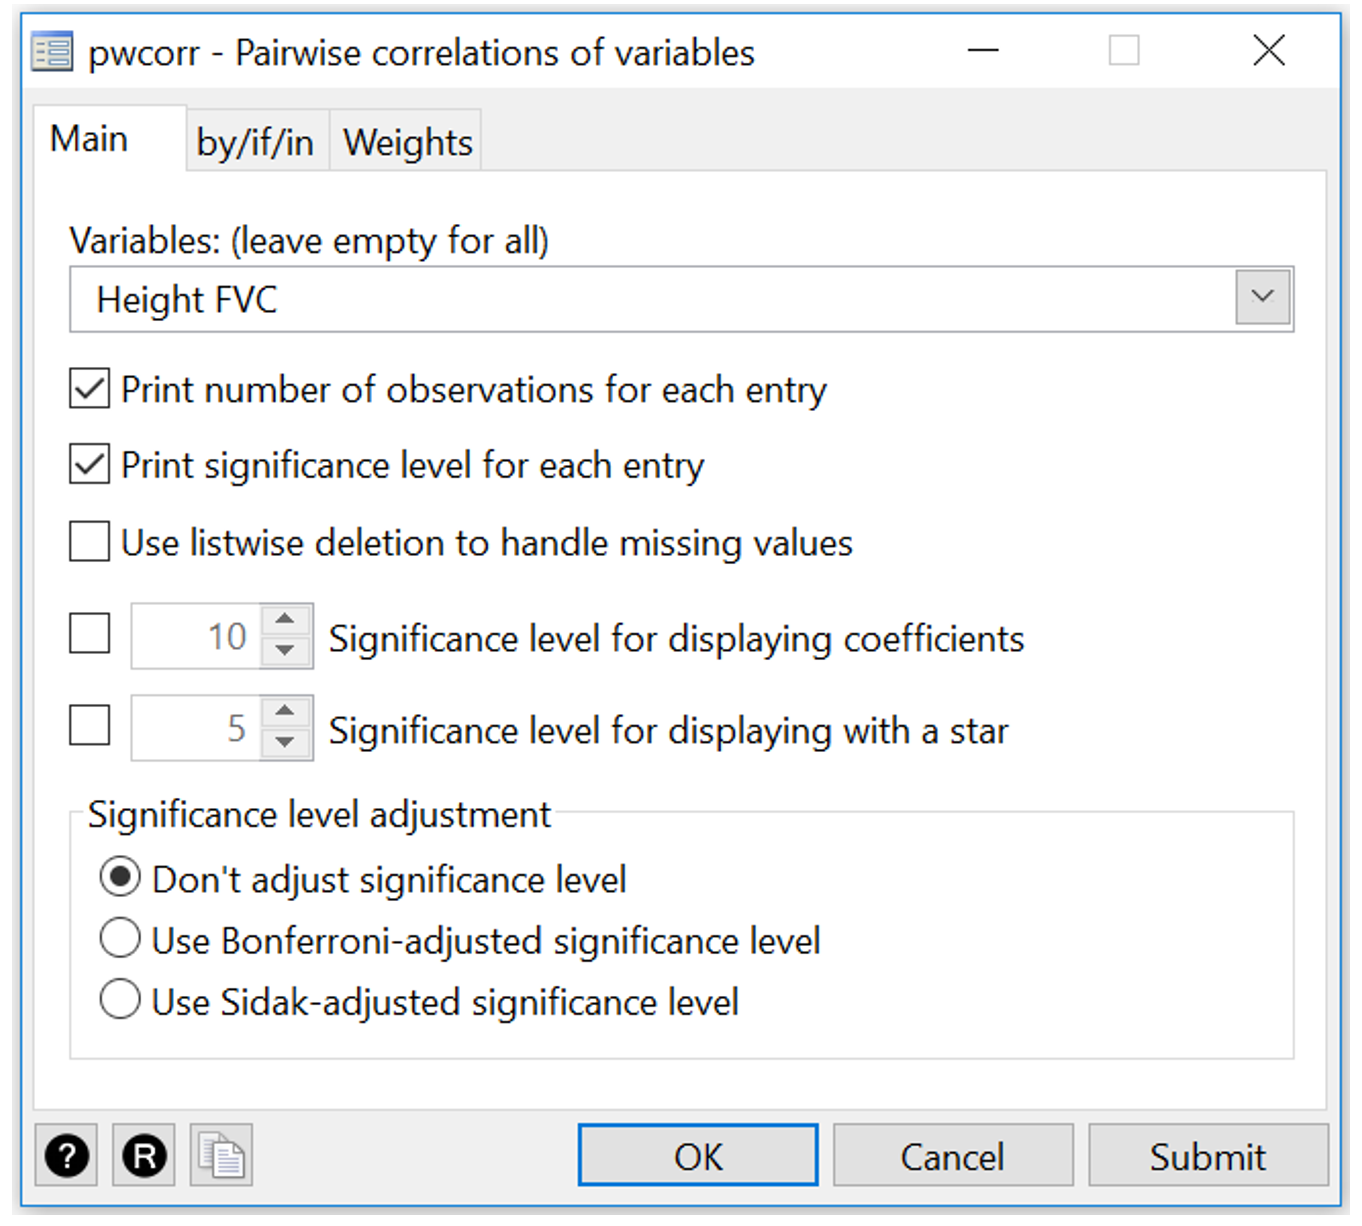
\includegraphics[width=0.66\linewidth]{img/mod08/stata/corr-1}

Click the \textbf{OK} or the \textbf{Submit} button when you are done to produce \textbf{Output 8.1},

{[}Command: \texttt{pwcorr\ Height\ FVC,\ obs\ sig}{]}

\hypertarget{fitting-a-simple-linear-regression-model}{%
\section{Fitting a simple linear regression model}\label{fitting-a-simple-linear-regression-model}}

We will fit a simple linear regression model with \texttt{Example\_8.1.dta} to quantify the relationship between FVC and height.

Choose \textbf{Statistics \textgreater{} Linear models and related \textgreater{} Linear regression}

In the \texttt{regress} dialog box, select \texttt{FVC} as the \textbf{Dependent variable}, and \texttt{Height} as the \textbf{Independent variable}.

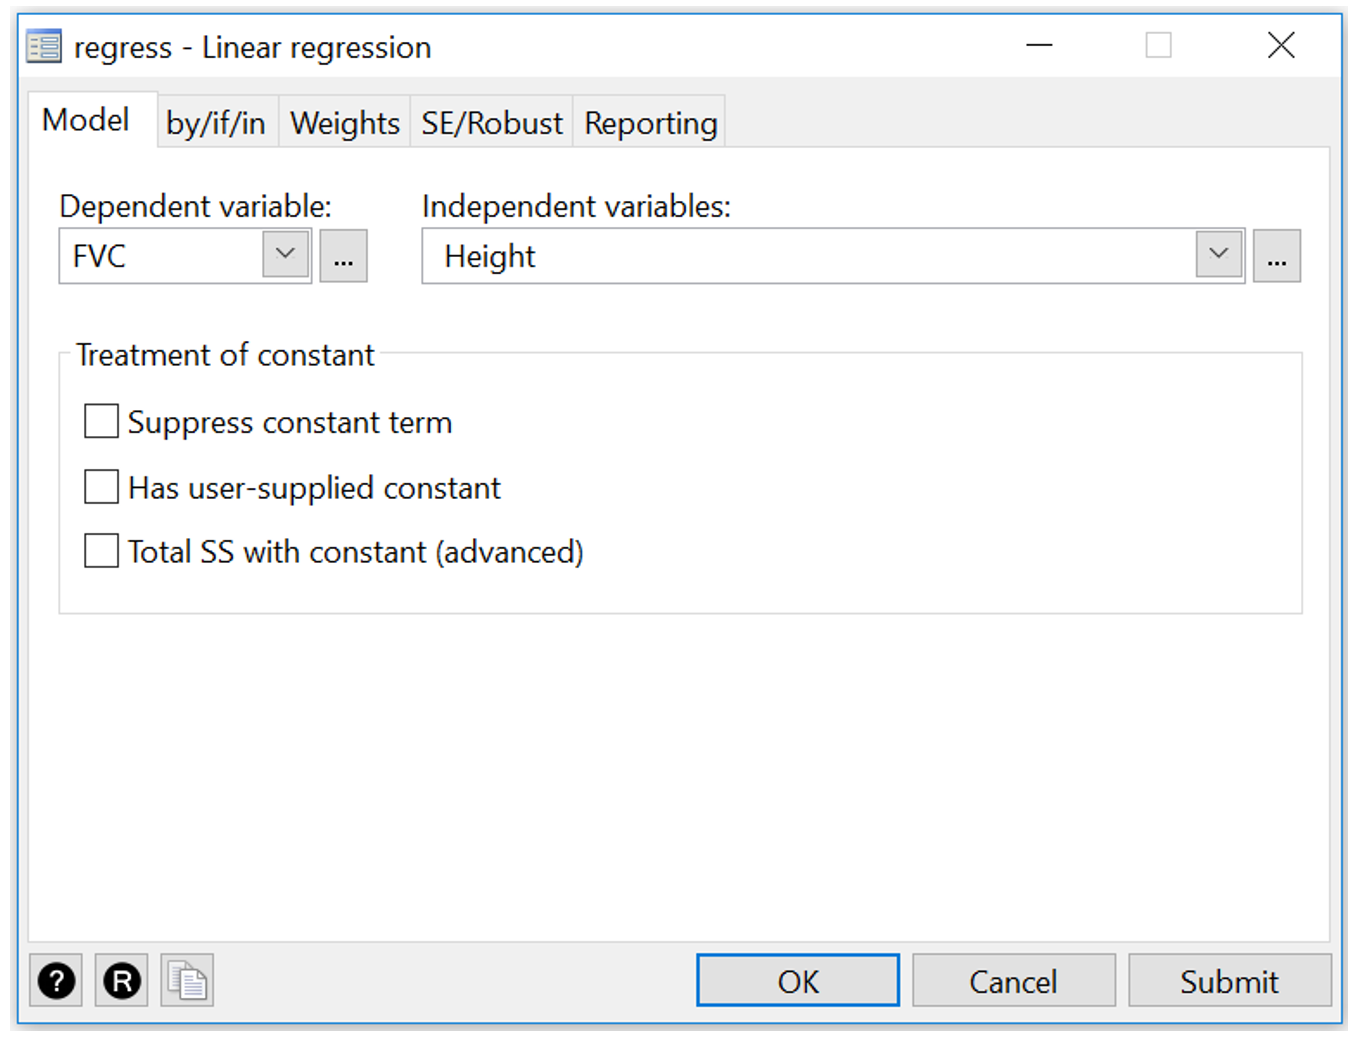
\includegraphics[width=0.66\linewidth]{img/mod08/stata/regr-1}

Click the \textbf{OK} or the \textbf{Submit} button when you are done to produce \textbf{Outputs 8.2 and 8.3}.

{[}Command: \texttt{reg\ FVC\ Height}{]}

\hypertarget{plotting-residuals-from-a-simple-linear-regression}{%
\section{Plotting residuals from a simple linear regression}\label{plotting-residuals-from-a-simple-linear-regression}}

To obtain the residuals, go to \textbf{Statistics \textgreater{} Post estimation} after running the regress command.

In the \texttt{Postestimation\ Selector} dialog box, select \textbf{Predictions and their SEs, leverage statistics, distance statistics, etc.} in the list under Predictions as shown below.

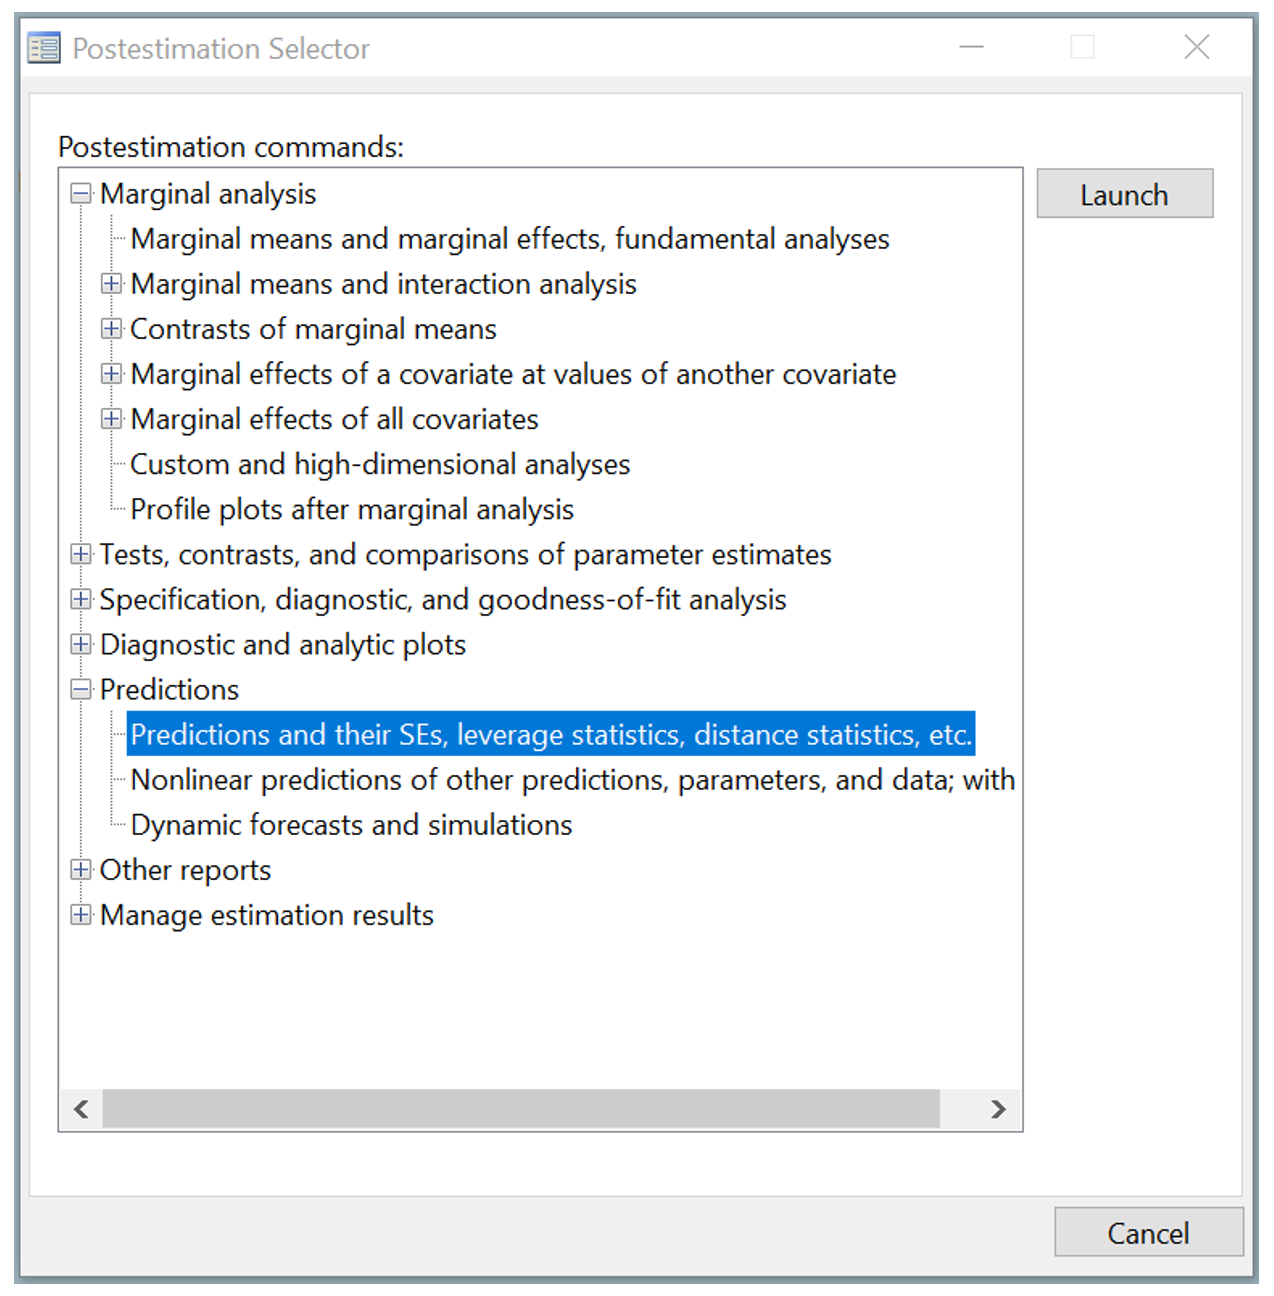
\includegraphics[width=0.66\linewidth]{img/mod08/stata/postest-1}

In the \texttt{predict} dialog box, choose the \textbf{Residuals} button and enter a New variable name (e.g.~\texttt{FVC\_resid}) for the residuals from the regression model.

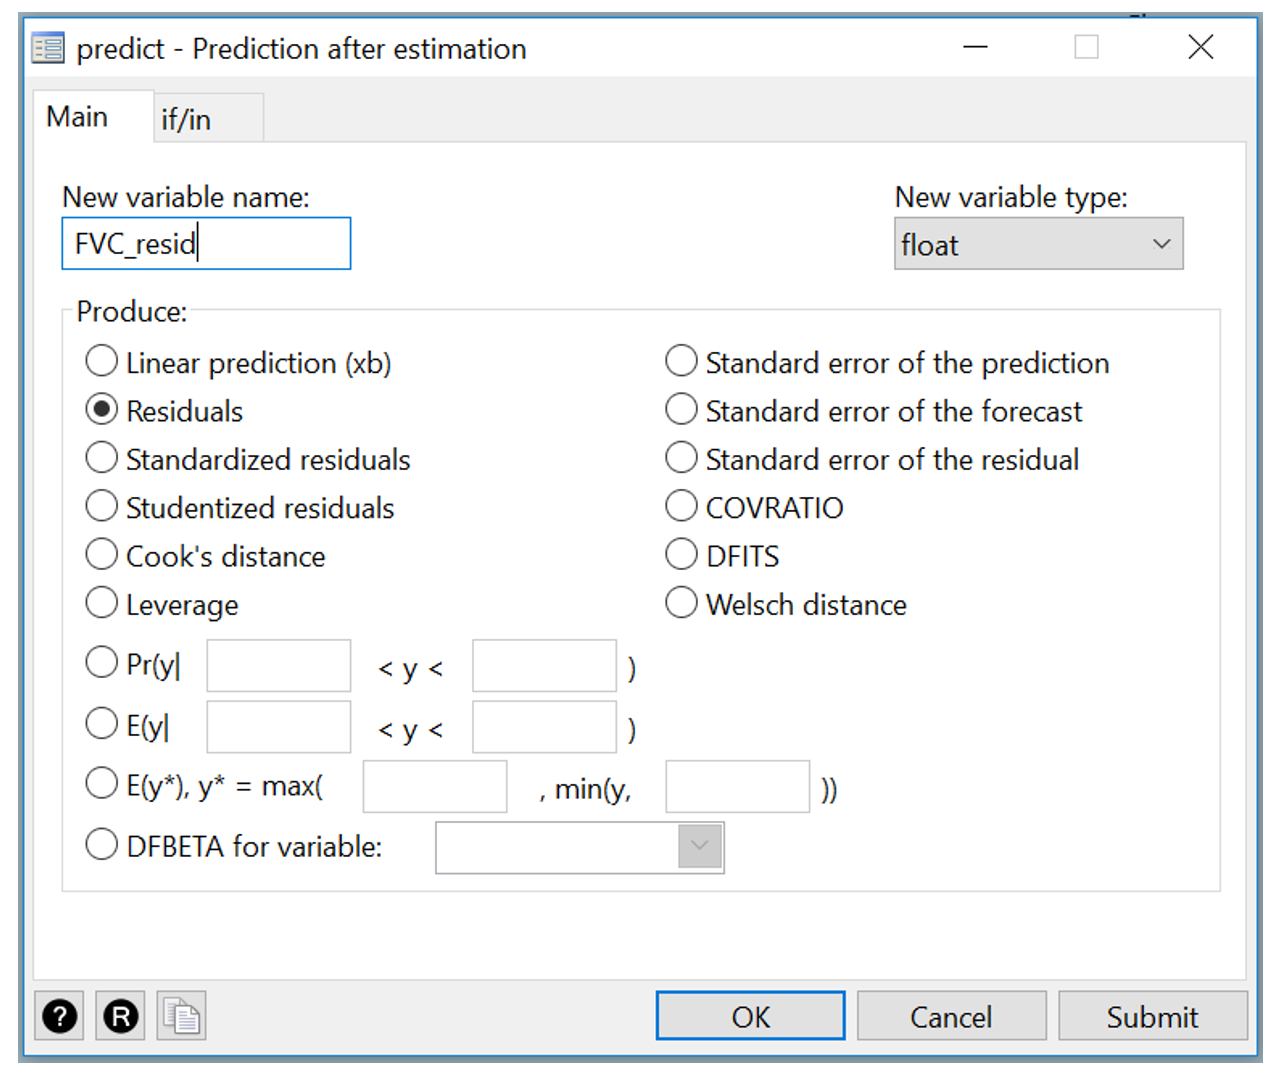
\includegraphics[width=0.66\linewidth]{img/mod08/stata/postest-2}

Click \textbf{OK} button when you are done.

{[}Command: \texttt{predict\ FVC\_resid,\ residuals}{]}

You can now check the assumption that the residuals are normally distributed by creating a histogram with the normal curve using \textbf{Graphics \textgreater{} Histogram} as shown in \textbf{Stata Notes} section for \textbf{Module 2}. Below is the \textbf{histogram} dialog box used to produce the graph in \textbf{Figure 8.5}.

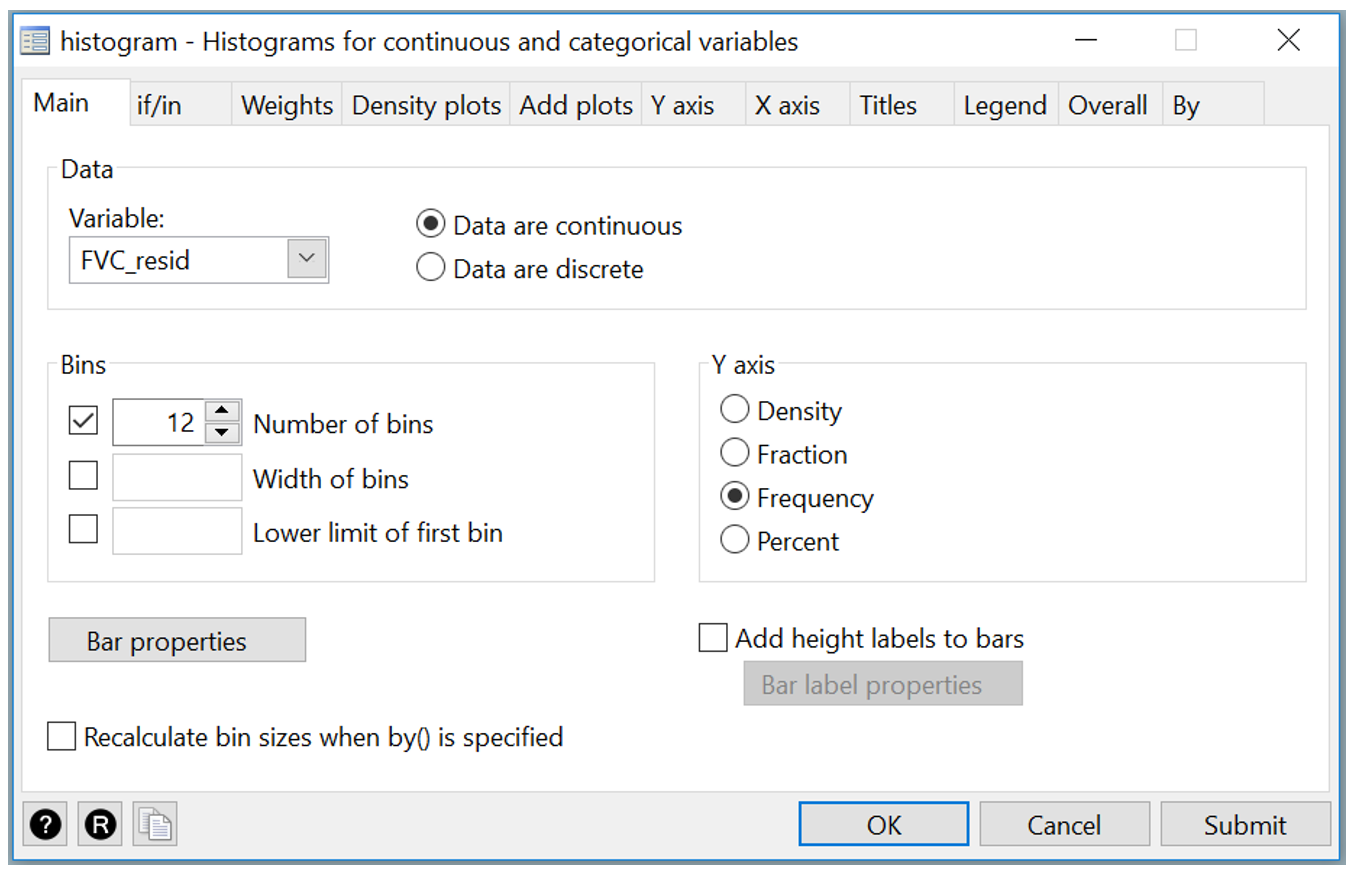
\includegraphics[width=0.66\linewidth]{img/mod08/stata/postest-3}

{[}Command: \texttt{histogram\ FVC\_resid,\ bin(12)\ frequency\ normal}{]}

\hypertarget{correlation-and-simple-linear-regression}{%
\chapter{Correlation and simple linear regression}\label{correlation-and-simple-linear-regression}}

\begin{Shaded}
\begin{Highlighting}[]
\FunctionTok{library}\NormalTok{(ggformula)}
\end{Highlighting}
\end{Shaded}

\begin{verbatim}
## Loading required package: ggstance
\end{verbatim}

\begin{verbatim}
## 
## Attaching package: 'ggstance'
\end{verbatim}

\begin{verbatim}
## The following objects are masked from 'package:ggplot2':
## 
##     geom_errorbarh, GeomErrorbarh
\end{verbatim}

\begin{verbatim}
## Loading required package: scales
\end{verbatim}

\begin{verbatim}
## 
## Attaching package: 'scales'
\end{verbatim}

\begin{verbatim}
## The following object is masked from 'package:huxtable':
## 
##     number_format
\end{verbatim}

\begin{verbatim}
## The following object is masked from 'package:purrr':
## 
##     discard
\end{verbatim}

\begin{verbatim}
## The following object is masked from 'package:readr':
## 
##     col_factor
\end{verbatim}

\begin{verbatim}
## Loading required package: ggridges
\end{verbatim}

\begin{verbatim}
## 
## New to ggformula?  Try the tutorials: 
##  learnr::run_tutorial("introduction", package = "ggformula")
##  learnr::run_tutorial("refining", package = "ggformula")
\end{verbatim}

We will demonstrate using R for correlation and simple linear regression using the dataset \texttt{Example\_8.1.csv}.

\begin{Shaded}
\begin{Highlighting}[]
\NormalTok{lung }\OtherTok{\textless{}{-}} \FunctionTok{read.csv}\NormalTok{(}\StringTok{"data/examples/Example\_8.1.csv"}\NormalTok{)}
\end{Highlighting}
\end{Shaded}

\hypertarget{creating-a-scatter-plot-1}{%
\section{Creating a scatter plot}\label{creating-a-scatter-plot-1}}

We can use the \texttt{plot} function to create a scatter plot to explore the association between height and FVC, assigning meaningful labels with the \texttt{xlab} and \texttt{ylab} commands:

\begin{Shaded}
\begin{Highlighting}[]
\FunctionTok{plot}\NormalTok{(}\AttributeTok{x=}\NormalTok{lung}\SpecialCharTok{$}\NormalTok{Height, }\AttributeTok{y=}\NormalTok{lung}\SpecialCharTok{$}\NormalTok{FVC, }
     \AttributeTok{xlab=}\StringTok{"Height (cm)"}\NormalTok{, }
     \AttributeTok{ylab=}\StringTok{"Forced vital capacity (L)"}\NormalTok{)}
\end{Highlighting}
\end{Shaded}

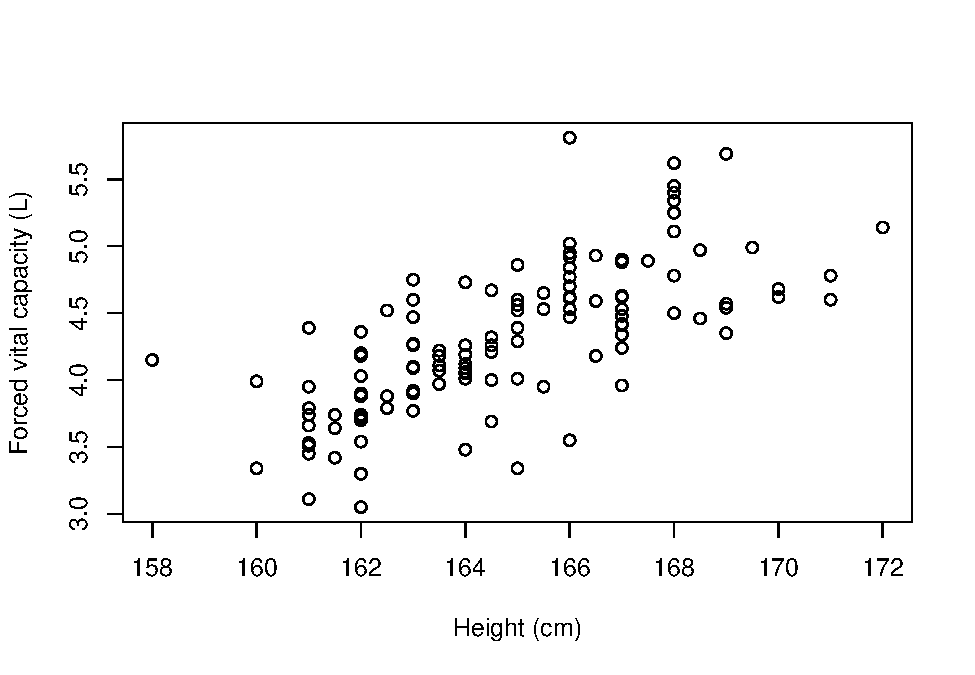
\includegraphics{PHCM9795_files/figure-latex/unnamed-chunk-3-1.pdf}

To add a fitted line, we can use the \texttt{abline()} function which adds a straight line to the plot. The equation of this straight line will be determined from the estimated regression line, which we specify with the \texttt{lm()} function, which fits a \emph{linear model}.

The basic syntax of the \texttt{lm()} function is: \texttt{lm(y\ \textasciitilde{}\ x)} where \texttt{y} represents the \emph{outcome} variable, and \texttt{x} represents the \emph{explanatory} variable. Putting this all together:

\begin{Shaded}
\begin{Highlighting}[]
\FunctionTok{plot}\NormalTok{(}\AttributeTok{x=}\NormalTok{lung}\SpecialCharTok{$}\NormalTok{Height, }\AttributeTok{y=}\NormalTok{lung}\SpecialCharTok{$}\NormalTok{FVC,}
     \AttributeTok{xlab=}\StringTok{"Height (cm)"}\NormalTok{,}
     \AttributeTok{ylab=}\StringTok{"Forced vital capacity (L)"}\NormalTok{)}

\FunctionTok{abline}\NormalTok{(}\FunctionTok{lm}\NormalTok{(lung}\SpecialCharTok{$}\NormalTok{FVC }\SpecialCharTok{\textasciitilde{}}\NormalTok{ lung}\SpecialCharTok{$}\NormalTok{Height))}
\end{Highlighting}
\end{Shaded}

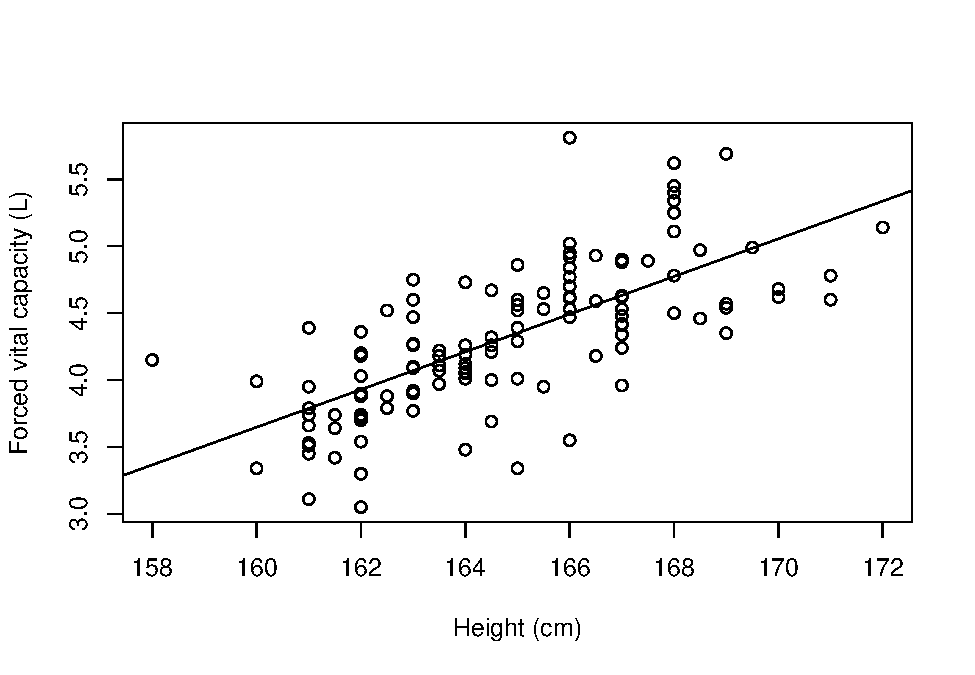
\includegraphics{PHCM9795_files/figure-latex/unnamed-chunk-4-1.pdf}

Or using the \texttt{ggformula} package, we form the basic plot using the following:

\begin{Shaded}
\begin{Highlighting}[]
\FunctionTok{gf\_point}\NormalTok{(FVC }\SpecialCharTok{\textasciitilde{}}\NormalTok{ Height, }\AttributeTok{data=}\NormalTok{lung,}
     \AttributeTok{xlab=}\StringTok{"Height (cm)"}\NormalTok{, }
     \AttributeTok{ylab=}\StringTok{"Forced vital capacity (L)"}\NormalTok{) }\SpecialCharTok{|\textgreater{}}
  \FunctionTok{gf\_theme}\NormalTok{(}\AttributeTok{theme =} \FunctionTok{theme\_minimal}\NormalTok{())}
\end{Highlighting}
\end{Shaded}

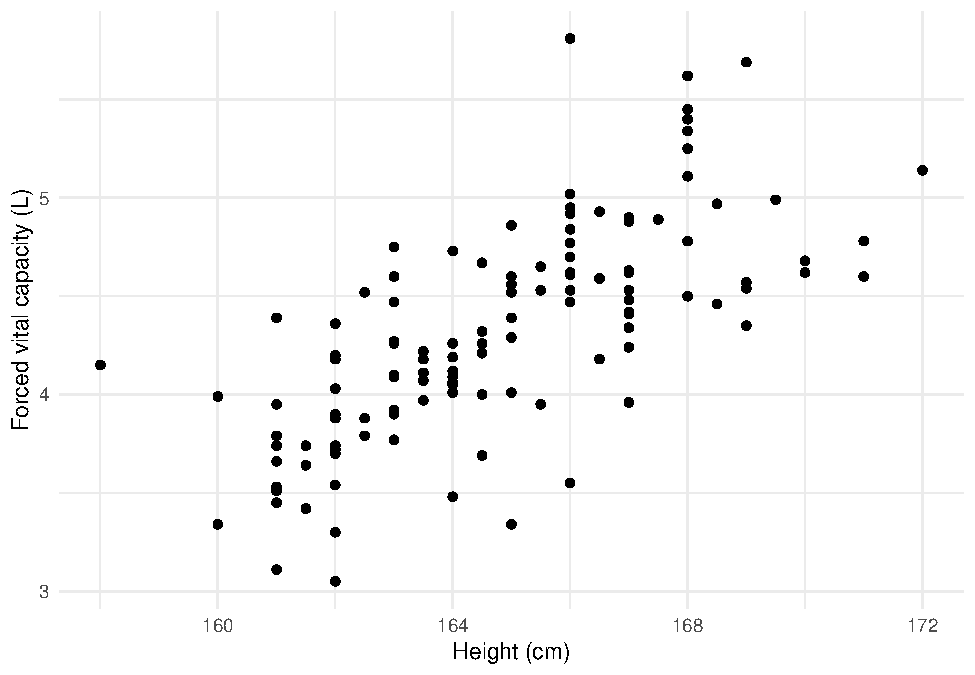
\includegraphics{PHCM9795_files/figure-latex/unnamed-chunk-5-1.pdf}

We can add an estimated linear regression line by piping the command \texttt{gf\_lm()}:

\begin{Shaded}
\begin{Highlighting}[]
\FunctionTok{gf\_point}\NormalTok{(FVC }\SpecialCharTok{\textasciitilde{}}\NormalTok{ Height, }\AttributeTok{data=}\NormalTok{lung,}
     \AttributeTok{xlab=}\StringTok{"Height (cm)"}\NormalTok{, }
     \AttributeTok{ylab=}\StringTok{"Forced vital capacity (L)"}\NormalTok{) }\SpecialCharTok{|\textgreater{}}
  \FunctionTok{gf\_lm}\NormalTok{() }\SpecialCharTok{|\textgreater{}}
  \FunctionTok{gf\_theme}\NormalTok{(}\AttributeTok{theme =} \FunctionTok{theme\_minimal}\NormalTok{())}
\end{Highlighting}
\end{Shaded}

\begin{verbatim}
## Warning: Using the `size` aesthietic with geom_line was deprecated in ggplot2 3.4.0.
## i Please use the `linewidth` aesthetic instead.
\end{verbatim}

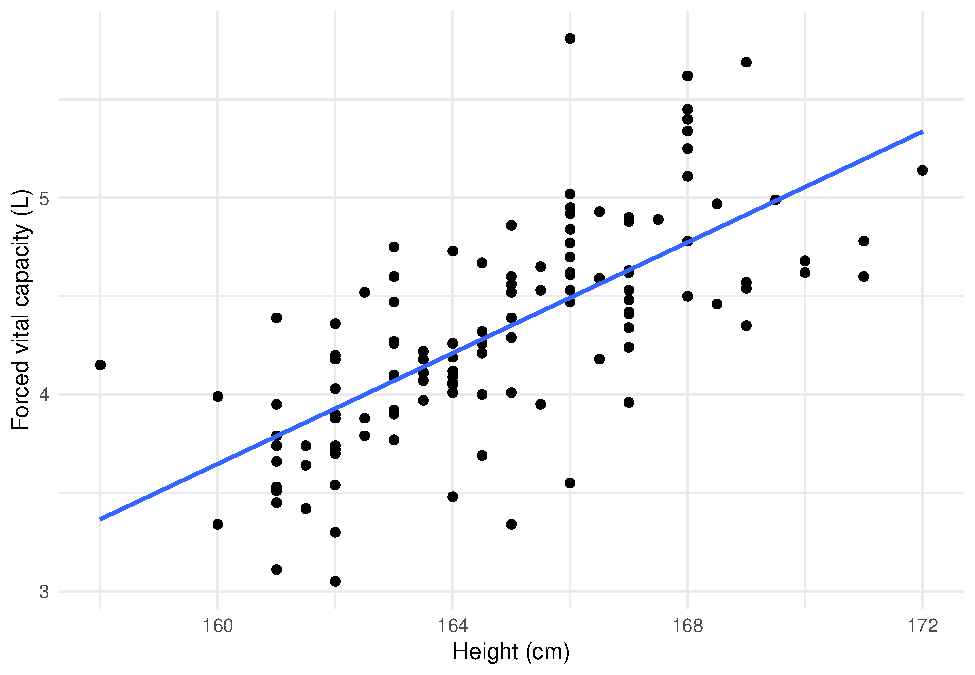
\includegraphics{PHCM9795_files/figure-latex/unnamed-chunk-6-1.pdf}

\hypertarget{calculating-a-correlation-coefficient-1}{%
\subsection*{Calculating a correlation coefficient}\label{calculating-a-correlation-coefficient-1}}
\addcontentsline{toc}{subsection}{Calculating a correlation coefficient}

We can use the \texttt{cor.test(x,\ y)} function to calculate a Pearson's correlation coefficient:

\begin{Shaded}
\begin{Highlighting}[]
\FunctionTok{cor.test}\NormalTok{(lung}\SpecialCharTok{$}\NormalTok{Height, lung}\SpecialCharTok{$}\NormalTok{FVC)}
\end{Highlighting}
\end{Shaded}

\begin{verbatim}
## 
##  Pearson's product-moment correlation
## 
## data:  lung$Height and lung$FVC
## t = 10.577, df = 118, p-value < 2.2e-16
## alternative hypothesis: true correlation is not equal to 0
## 95 percent confidence interval:
##  0.5924715 0.7794090
## sample estimates:
##       cor 
## 0.6976279
\end{verbatim}

\hypertarget{fitting-a-simple-linear-regression-model-1}{%
\section{Fitting a simple linear regression model}\label{fitting-a-simple-linear-regression-model-1}}

We can use the \texttt{lm} function to fit a simple linear regression model, specifying the model as \texttt{y\ \textasciitilde{}\ x} where \texttt{y} represents the \emph{outcome} variable, and \texttt{x} represents the \emph{explanatory} variable. Using \texttt{Example\_8.1.rds}, we can quantify the relationship between FVC and height:

\begin{Shaded}
\begin{Highlighting}[]
\FunctionTok{lm}\NormalTok{(lung}\SpecialCharTok{$}\NormalTok{FVC }\SpecialCharTok{\textasciitilde{}}\NormalTok{ lung}\SpecialCharTok{$}\NormalTok{Height)}
\end{Highlighting}
\end{Shaded}

\begin{verbatim}
## 
## Call:
## lm(formula = lung$FVC ~ lung$Height)
## 
## Coefficients:
## (Intercept)  lung$Height  
##    -18.8735       0.1408
\end{verbatim}

The default output from the \texttt{lm} function is rather sparse. We can obtain much more useful information by defining the linear regression model as an object, then using the \texttt{summary()} function:

\begin{Shaded}
\begin{Highlighting}[]
\NormalTok{model }\OtherTok{\textless{}{-}} \FunctionTok{lm}\NormalTok{(lung}\SpecialCharTok{$}\NormalTok{FVC }\SpecialCharTok{\textasciitilde{}}\NormalTok{ lung}\SpecialCharTok{$}\NormalTok{Height)}
\FunctionTok{summary}\NormalTok{(model)}
\end{Highlighting}
\end{Shaded}

\begin{verbatim}
## 
## Call:
## lm(formula = lung$FVC ~ lung$Height)
## 
## Residuals:
##      Min       1Q   Median       3Q      Max 
## -1.01139 -0.23643 -0.02082  0.24918  1.31786 
## 
## Coefficients:
##              Estimate Std. Error t value Pr(>|t|)    
## (Intercept) -18.87347    2.19365  -8.604 3.89e-14 ***
## lung$Height   0.14076    0.01331  10.577  < 2e-16 ***
## ---
## Signif. codes:  0 '***' 0.001 '**' 0.01 '*' 0.05 '.' 0.1 ' ' 1
## 
## Residual standard error: 0.3965 on 118 degrees of freedom
## Multiple R-squared:  0.4867, Adjusted R-squared:  0.4823 
## F-statistic: 111.9 on 1 and 118 DF,  p-value: < 2.2e-16
\end{verbatim}

Finally, we can obtain 95\% confidence intervals for the regression coefficients using the \texttt{confint} function:

\begin{Shaded}
\begin{Highlighting}[]
\FunctionTok{confint}\NormalTok{(model)}
\end{Highlighting}
\end{Shaded}

\begin{verbatim}
##                   2.5 %      97.5 %
## (Intercept) -23.2174967 -14.5294441
## lung$Height   0.1144042   0.1671092
\end{verbatim}

\hypertarget{plotting-residuals-from-a-simple-linear-regression-1}{%
\section{Plotting residuals from a simple linear regression}\label{plotting-residuals-from-a-simple-linear-regression-1}}

We can use the \texttt{resid} function to obtain the residuals from a saved model. These residuals can then be plotted using a histogram in the usual way:

\begin{Shaded}
\begin{Highlighting}[]
\NormalTok{residuals }\OtherTok{\textless{}{-}} \FunctionTok{resid}\NormalTok{(model)}
\FunctionTok{hist}\NormalTok{(residuals)}
\end{Highlighting}
\end{Shaded}

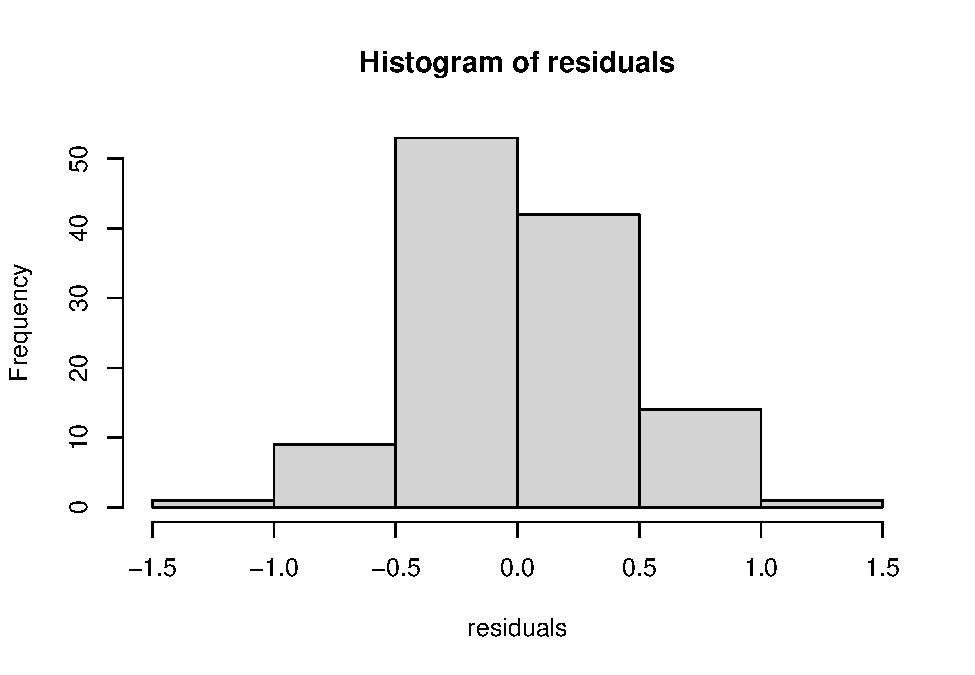
\includegraphics{PHCM9795_files/figure-latex/unnamed-chunk-11-1.pdf}

A Normal curve can be overlaid if we plot the residuals using a probability scale.

\begin{Shaded}
\begin{Highlighting}[]
\FunctionTok{hist}\NormalTok{(residuals, }\AttributeTok{probability =} \ConstantTok{TRUE}\NormalTok{,}
     \AttributeTok{ylim =} \FunctionTok{c}\NormalTok{(}\DecValTok{0}\NormalTok{, }\DecValTok{1}\NormalTok{))}

\FunctionTok{curve}\NormalTok{(}\FunctionTok{dnorm}\NormalTok{(x, }\AttributeTok{mean=}\FunctionTok{mean}\NormalTok{(residuals), }\AttributeTok{sd=}\FunctionTok{sd}\NormalTok{(residuals)), }
      \AttributeTok{col=}\StringTok{"darkblue"}\NormalTok{, }\AttributeTok{lwd=}\DecValTok{2}\NormalTok{, }\AttributeTok{add=}\ConstantTok{TRUE}\NormalTok{)}
\end{Highlighting}
\end{Shaded}

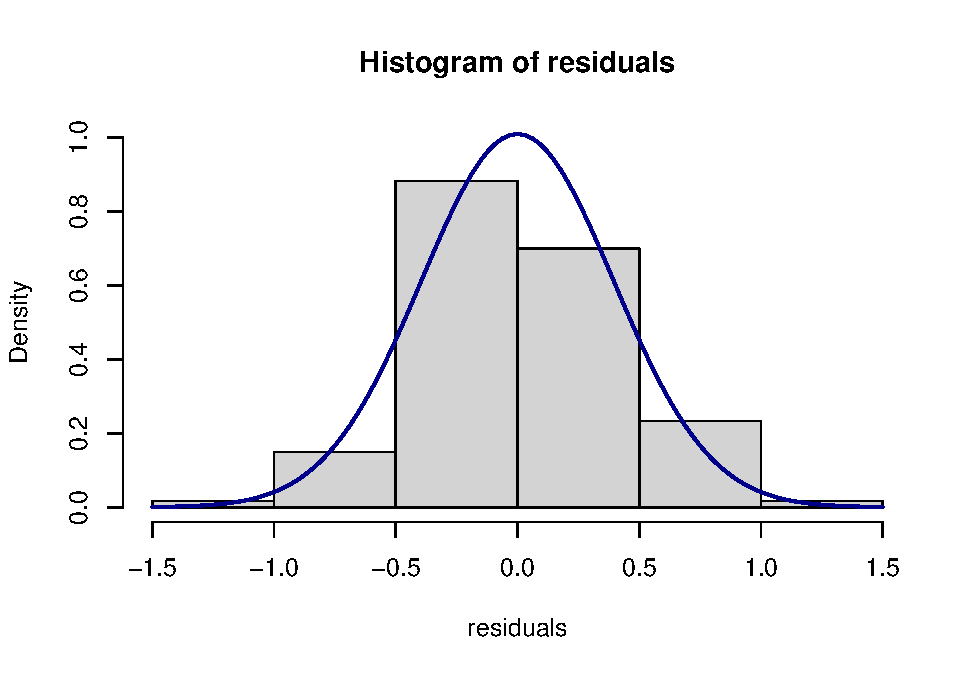
\includegraphics{PHCM9795_files/figure-latex/unnamed-chunk-12-1.pdf}

Using \texttt{ggformula}, we can plot the residuals as a histogram:

\begin{Shaded}
\begin{Highlighting}[]
\FunctionTok{gf\_dhistogram}\NormalTok{(}\SpecialCharTok{\textasciitilde{}}\NormalTok{ residuals, }\AttributeTok{data=}\NormalTok{model) }\SpecialCharTok{|\textgreater{}}
  \FunctionTok{gf\_dist}\NormalTok{(}\StringTok{"norm"}\NormalTok{, }
          \AttributeTok{params=}\FunctionTok{list}\NormalTok{(}\AttributeTok{mean=}\FunctionTok{mean}\NormalTok{(model}\SpecialCharTok{$}\NormalTok{residuals), }
                      \AttributeTok{sd=}\FunctionTok{sd}\NormalTok{(model}\SpecialCharTok{$}\NormalTok{residuals)))}
\end{Highlighting}
\end{Shaded}

\begin{verbatim}
## Warning: `stat(density)` was deprecated in ggplot2 3.4.0.
## i Please use `after_stat(density)` instead.
\end{verbatim}

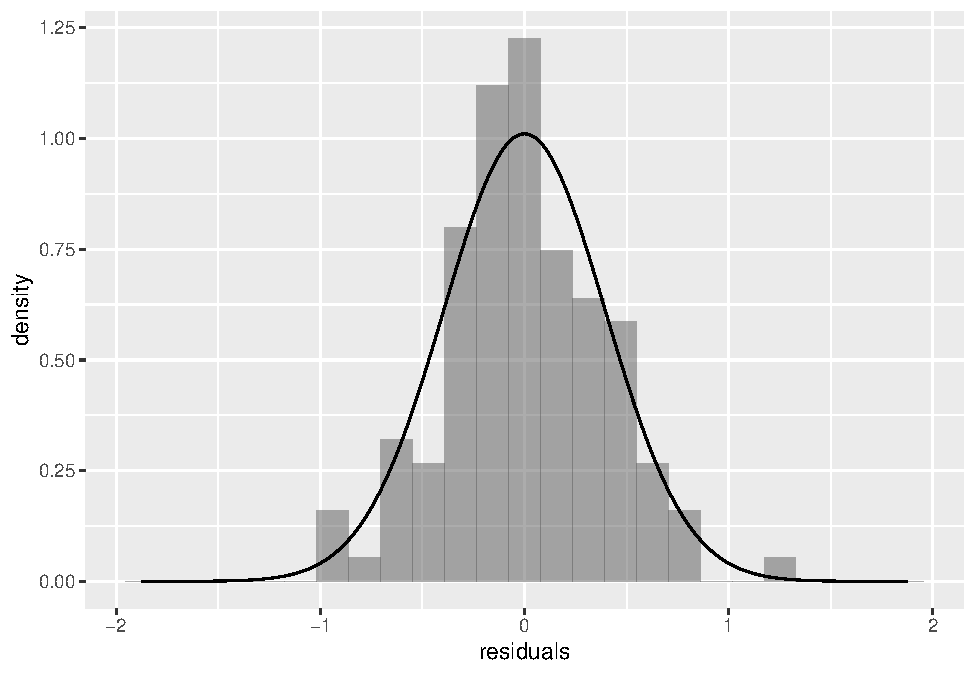
\includegraphics{PHCM9795_files/figure-latex/unnamed-chunk-13-1.pdf}

\begin{Shaded}
\begin{Highlighting}[]
\FunctionTok{gf\_dhistogram}\NormalTok{(}\SpecialCharTok{\textasciitilde{}}\NormalTok{ residuals, }\AttributeTok{data=}\NormalTok{model) }\SpecialCharTok{|\textgreater{}}
  \FunctionTok{gf\_dens}\NormalTok{()}
\end{Highlighting}
\end{Shaded}

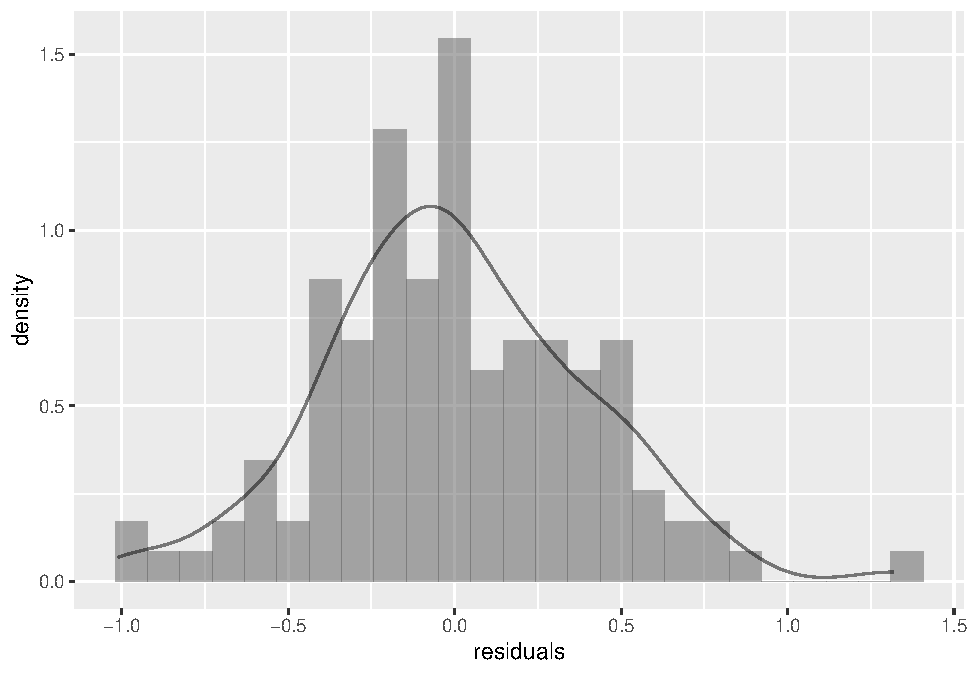
\includegraphics{PHCM9795_files/figure-latex/unnamed-chunk-13-2.pdf}

\hypertarget{learning-activities}{%
\chapter*{\texorpdfstring{\textbf{8} Learning Activities}{8 Learning Activities}}\label{learning-activities}}
\addcontentsline{toc}{chapter}{\textbf{8} Learning Activities}

\hypertarget{activity-8.1}{%
\subsection*{Activity 8.1}\label{activity-8.1}}
\addcontentsline{toc}{subsection}{Activity 8.1}

To investigate how body weight (kg) effects blood plasma volume (mL), data were collected from 30 participants and a simple linear regression analysis was conducted. The slope of the regression was 68 (95\% confidence interval 52 to 84) and the intercept was −1570 (95\% confidence interval −2655 to −492).

{[}\emph{You do not need Stata for this Activity}{]}

\begin{enumerate}
\def\labelenumi{\alph{enumi})}
\tightlist
\item
  What is the outcome variable and explanatory (exposure) variable?
\item
  Interpret the regression slope and its 95\% CI
\item
  Write the regression equation
\item
  If we randomly sampled a person from the population and found that their weight is 80kg, what would be the predicted value of plasma volume for this person?
\end{enumerate}

\hypertarget{activity-8.2}{%
\subsection*{Activity 8.2}\label{activity-8.2}}
\addcontentsline{toc}{subsection}{Activity 8.2}

To examine whether age predicts IQ, data were collected on 104 people. Use the data in the Stata file \texttt{Activity\_8.2.dta} to answer the following questions.

\begin{enumerate}
\def\labelenumi{\alph{enumi})}
\tightlist
\item
  What are the outcome variable and the explanatory variable?
\item
  Create a scatter plot with the two variables. What can you infer from the scatter plot?
\item
  Using Stata, obtain the correlation coefficient between age and IQ and interpret it.
\item
  Conduct a simple linear regression using Stata and report the relationship between the two variables including the interpretation of the R2 value. Are the assumptions for linear regression met in this model?
\item
  What could you infer about the association between age and IQ in the population, based on the results of the regression analysis in this sample?
\end{enumerate}

\hypertarget{activity-8.3}{%
\subsection*{Activity 8.3}\label{activity-8.3}}
\addcontentsline{toc}{subsection}{Activity 8.3}

Which of the following correlation coefficients indicates the weakest linear relationship and why?

\begin{enumerate}
\def\labelenumi{\alph{enumi})}
\tightlist
\item
  r = 0.72
\item
  r = 0.41
\item
  r = 0.13
\item
  r = −0.33
\item
  r = −0.84
\end{enumerate}

\hypertarget{activity-8.4}{%
\subsection*{Activity 8.4}\label{activity-8.4}}
\addcontentsline{toc}{subsection}{Activity 8.4}

Are the following statements true or false?

\begin{enumerate}
\def\labelenumi{\alph{enumi})}
\tightlist
\item
  If a correlation coefficient is closer to 1.00 than to 0.00, this indicates that the outcome is caused by the exposure.
\item
  If a researcher has data on two variables, there will be a higher correlation if the two means are close together and a lower correlation if the two means are far apart.
\end{enumerate}

  \bibliography{PHCM9795.bib}

\end{document}
